
%% bare_conf.tex
%% V1.4a
%% 2014/09/17
%% by Michael Shell
%% See:
%% http://www.michaelshell.org/
%% for current contact information.
%%
%% This is a skeleton file demonstrating the use of IEEEtran.cls
%% (requires IEEEtran.cls version 1.8a or later) with an IEEE
%% conference paper.
%%
%% Support sites:
%% http://www.michaelshell.org/tex/ieeetran/
%% http://www.ctan.org/tex-archive/macros/latex/contrib/IEEEtran/
%% and
%% http://www.ieee.org/

%%*************************************************************************
%% Legal Notice:
%% This code is offered as-is without any warranty either expressed or
%% implied; without even the implied warranty of MERCHANTABILITY or
%% FITNESS FOR A PARTICULAR PURPOSE!
%% User assumes all risk.
%% In no event shall IEEE or any contributor to this code be liable for
%% any damages or losses, including, but not limited to, incidental,
%% consequential, or any other damages, resulting from the use or misuse
%% of any information contained here.
%%
%% All comments are the opinions of their respective authors and are not
%% necessarily endorsed by the IEEE.
%%
%% This work is distributed under the LaTeX Project Public License (LPPL)
%% ( http://www.latex-project.org/ ) version 1.3, and may be freely used,
%% distributed and modified. A copy of the LPPL, version 1.3, is included
%% in the base LaTeX documentation of all distributions of LaTeX released
%% 2003/12/01 or later.
%% Retain all contribution notices and credits.
%% ** Modified files should be clearly indicated as such, including  **
%% ** renaming them and changing author support contact information. **
%%
%% File list of work: IEEEtran.cls, IEEEtran_HOWTO.pdf, bare_adv.tex,
%%                    bare_conf.tex, bare_jrnl.tex, bare_conf_compsoc.tex,
%%                    bare_jrnl_compsoc.tex, bare_jrnl_transmag.tex
%%*************************************************************************


% *** Authors should verify (and, if needed, correct) their LaTeX system  ***
% *** with the testflow diagnostic prior to trusting their LaTeX platform ***
% *** with production work. IEEE's font choices and paper sizes can       ***
% *** trigger bugs that do not appear when using other class files.       ***                          ***
% The testflow support page is at:
% http://www.michaelshell.org/tex/testflow/



\documentclass[conference]{IEEEtran}
% Some Computer Society conferences also require the compsoc mode option,
% but others use the standard conference format.
%
% If IEEEtran.cls has not been installed into the LaTeX system files,
% manually specify the path to it like:
% \documentclass[conference]{../sty/IEEEtran}





% Some very useful LaTeX packages include:
% (uncomment the ones you want to load)


% *** MISC UTILITY PACKAGES ***
%
%\usepackage{ifpdf}
% Heiko Oberdiek's ifpdf.sty is very useful if you need conditional
% compilation based on whether the output is pdf or dvi.
% usage:
% \ifpdf
%   % pdf code
% \else
%   % dvi code
% \fi
% The latest version of ifpdf.sty can be obtained from:
% http://www.ctan.org/tex-archive/macros/latex/contrib/oberdiek/
% Also, note that IEEEtran.cls V1.7 and later provides a builtin
% \ifCLASSINFOpdf conditional that works the same way.
% When switching from latex to pdflatex and vice-versa, the compiler may
% have to be run twice to clear warning/error messages.






% *** CITATION PACKAGES ***
%
%\usepackage{cite}
% cite.sty was written by Donald Arseneau
% V1.6 and later of IEEEtran pre-defines the format of the cite.sty package
% \cite{} output to follow that of IEEE. Loading the cite package will
% result in citation numbers being automatically sorted and properly
% "compressed/ranged". e.g., [1], [9], [2], [7], [5], [6] without using
% cite.sty will become [1], [2], [5]--[7], [9] using cite.sty. cite.sty's
% \cite will automatically add leading space, if needed. Use cite.sty's
% noadjust option (cite.sty V3.8 and later) if you want to turn this off
% such as if a citation ever needs to be enclosed in parenthesis.
% cite.sty is already installed on most LaTeX systems. Be sure and use
% version 5.0 (2009-03-20) and later if using hyperref.sty.
% The latest version can be obtained at:
% http://www.ctan.org/tex-archive/macros/latex/contrib/cite/
% The documentation is contained in the cite.sty file itself.






% *** GRAPHICS RELATED PACKAGES ***
%
\ifCLASSINFOpdf
  % \usepackage[pdftex]{graphicx}
  % declare the path(s) where your graphic files are
  % \graphicspath{{../pdf/}{../jpeg/}}
  % and their extensions so you won't have to specify these with
  % every instance of \includegraphics
  % \DeclareGraphicsExtensions{.pdf,.jpeg,.png}
\else
  % or other class option (dvipsone, dvipdf, if not using dvips). graphicx
  % will default to the driver specified in the system graphics.cfg if no
  % driver is specified.
  % \usepackage[dvips]{graphicx}
  % declare the path(s) where your graphic files are
  % \graphicspath{{../eps/}}
  % and their extensions so you won't have to specify these with
  % every instance of \includegraphics
  % \DeclareGraphicsExtensions{.eps}
\fi
% graphicx was written by David Carlisle and Sebastian Rahtz. It is
% required if you want graphics, photos, etc. graphicx.sty is already
% installed on most LaTeX systems. The latest version and documentation
% can be obtained at:
% http://www.ctan.org/tex-archive/macros/latex/required/graphics/
% Another good source of documentation is "Using Imported Graphics in
% LaTeX2e" by Keith Reckdahl which can be found at:
% http://www.ctan.org/tex-archive/info/epslatex/
%
% latex, and pdflatex in dvi mode, support graphics in encapsulated
% postscript (.eps) format. pdflatex in pdf mode supports graphics
% in .pdf, .jpeg, .png and .mps (metapost) formats. Users should ensure
% that all non-photo figures use a vector format (.eps, .pdf, .mps) and
% not a bitmapped formats (.jpeg, .png). IEEE frowns on bitmapped formats
% which can result in "jaggedy"/blurry rendering of lines and letters as
% well as large increases in file sizes.
%
% You can find documentation about the pdfTeX application at:
% http://www.tug.org/applications/pdftex





% *** MATH PACKAGES ***
%
%\usepackage[cmex10]{amsmath}
% A popular package from the American Mathematical Society that provides
% many useful and powerful commands for dealing with mathematics. If using
% it, be sure to load this package with the cmex10 option to ensure that
% only type 1 fonts will utilized at all point sizes. Without this option,
% it is possible that some math symbols, particularly those within
% footnotes, will be rendered in bitmap form which will result in a
% document that can not be IEEE Xplore compliant!
%
% Also, note that the amsmath package sets \interdisplaylinepenalty to 10000
% thus preventing page breaks from occurring within multiline equations. Use:
%\interdisplaylinepenalty=2500
% after loading amsmath to restore such page breaks as IEEEtran.cls normally
% does. amsmath.sty is already installed on most LaTeX systems. The latest
% version and documentation can be obtained at:
% http://www.ctan.org/tex-archive/macros/latex/required/amslatex/math/





% *** SPECIALIZED LIST PACKAGES ***
%
%\usepackage{algorithmic}
% algorithmic.sty was written by Peter Williams and Rogerio Brito.
% This package provides an algorithmic environment fo describing algorithms.
% You can use the algorithmic environment in-text or within a figure
% environment to provide for a floating algorithm. Do NOT use the algorithm
% floating environment provided by algorithm.sty (by the same authors) or
% algorithm2e.sty (by Christophe Fiorio) as IEEE does not use dedicated
% algorithm float types and packages that provide these will not provide
% correct IEEE style captions. The latest version and documentation of
% algorithmic.sty can be obtained at:
% http://www.ctan.org/tex-archive/macros/latex/contrib/algorithms/
% There is also a support site at:
% http://algorithms.berlios.de/index.html
% Also of interest may be the (relatively newer and more customizable)
% algorithmicx.sty package by Szasz Janos:
% http://www.ctan.org/tex-archive/macros/latex/contrib/algorithmicx/




% *** ALIGNMENT PACKAGES ***
%
%\usepackage{array}
% Frank Mittelbach's and David Carlisle's array.sty patches and improves
% the standard LaTeX2e array and tabular environments to provide better
% appearance and additional user controls. As the default LaTeX2e table
% generation code is lacking to the point of almost being broken with
% respect to the quality of the end results, all users are strongly
% advised to use an enhanced (at the very least that provided by array.sty)
% set of table tools. array.sty is already installed on most systems. The
% latest version and documentation can be obtained at:
% http://www.ctan.org/tex-archive/macros/latex/required/tools/


% IEEEtran contains the IEEEeqnarray family of commands that can be used to
% generate multiline equations as well as matrices, tables, etc., of high
% quality.




% *** SUBFIGURE PACKAGES ***
%\ifCLASSOPTIONcompsoc
%  \usepackage[caption=false,font=normalsize,labelfont=sf,textfont=sf]{subfig}
%\else
%  \usepackage[caption=false,font=footnotesize]{subfig}
%\fi
% subfig.sty, written by Steven Douglas Cochran, is the modern replacement
% for subfigure.sty, the latter of which is no longer maintained and is
% incompatible with some LaTeX packages including fixltx2e. However,
% subfig.sty requires and automatically loads Axel Sommerfeldt's caption.sty
% which will override IEEEtran.cls' handling of captions and this will result
% in non-IEEE style figure/table captions. To prevent this problem, be sure
% and invoke subfig.sty's "caption=false" package option (available since
% subfig.sty version 1.3, 2005/06/28) as this is will preserve IEEEtran.cls
% handling of captions.
% Note that the Computer Society format requires a larger sans serif font
% than the serif footnote size font used in traditional IEEE formatting
% and thus the need to invoke different subfig.sty package options depending
% on whether compsoc mode has been enabled.
%
% The latest version and documentation of subfig.sty can be obtained at:
% http://www.ctan.org/tex-archive/macros/latex/contrib/subfig/




% *** FLOAT PACKAGES ***
%
%\usepackage{fixltx2e}
% fixltx2e, the successor to the earlier fix2col.sty, was written by
% Frank Mittelbach and David Carlisle. This package corrects a few problems
% in the LaTeX2e kernel, the most notable of which is that in current
% LaTeX2e releases, the ordering of single and double column floats is not
% guaranteed to be preserved. Thus, an unpatched LaTeX2e can allow a
% single column figure to be placed prior to an earlier double column
% figure. The latest version and documentation can be found at:
% http://www.ctan.org/tex-archive/macros/latex/base/


%\usepackage{stfloats}
% stfloats.sty was written by Sigitas Tolusis. This package gives LaTeX2e
% the ability to do double column floats at the bottom of the page as well
% as the top. (e.g., "\begin{figure*}[!b]" is not normally possible in
% LaTeX2e). It also provides a command:
%\fnbelowfloat
% to enable the placement of footnotes below bottom floats (the standard
% LaTeX2e kernel puts them above bottom floats). This is an invasive package
% which rewrites many portions of the LaTeX2e float routines. It may not work
% with other packages that modify the LaTeX2e float routines. The latest
% version and documentation can be obtained at:
% http://www.ctan.org/tex-archive/macros/latex/contrib/sttools/
% Do not use the stfloats baselinefloat ability as IEEE does not allow
% \baselineskip to stretch. Authors submitting work to the IEEE should note
% that IEEE rarely uses double column equations and that authors should try
% to avoid such use. Do not be tempted to use the cuted.sty or midfloat.sty
% packages (also by Sigitas Tolusis) as IEEE does not format its papers in
% such ways.
% Do not attempt to use stfloats with fixltx2e as they are incompatible.
% Instead, use Morten Hogholm'a dblfloatfix which combines the features
% of both fixltx2e and stfloats:
%
% \usepackage{dblfloatfix}
% The latest version can be found at:
% http://www.ctan.org/tex-archive/macros/latex/contrib/dblfloatfix/




% *** PDF, URL AND HYPERLINK PACKAGES ***
%
%\usepackage{url}
% url.sty was written by Donald Arseneau. It provides better support for
% handling and breaking URLs. url.sty is already installed on most LaTeX
% systems. The latest version and documentation can be obtained at:
% http://www.ctan.org/tex-archive/macros/latex/contrib/url/
% Basically, \url{my_url_here}.




% *** Do not adjust lengths that control margins, column widths, etc. ***
% *** Do not use packages that alter fonts (such as pslatex).         ***
% There should be no need to do such things with IEEEtran.cls V1.6 and later.
% (Unless specifically asked to do so by the journal or conference you plan
% to submit to, of course. )


% correct bad hyphenation here
\hyphenation{op-tical net-works semi-conduc-tor}
%\hyphenation{op-tical net-works semi-conduc-tor}
\usepackage{mathrsfs}
\usepackage{amsmath}
\usepackage{amsfonts}
\usepackage{float}
\usepackage{graphicx}
\usepackage{algorithm}
\usepackage{algorithmic}
\usepackage{amsthm}
\usepackage{stfloats}
\usepackage{amsmath}
 \usepackage{setspace}
 \usepackage{bm}

\begin{document}
%
% paper title
% Titles are generally capitalized except for words such as a, an, and, as,
% at, but, by, for, in, nor, of, on, or, the, to and up, which are usually
% not capitalized unless they are the first or last word of the title.
% Linebreaks \\ can be used within to get better formatting as desired.
% Do not put math or special symbols in the title.
\title{Improved Spatially Coupled Multiuser Superposition Transmission via Constellation Rotation}


% author names and affiliations
% use a multiple column layout for up to three different
% affiliations
\author{\IEEEauthorblockN{Min Jiang and Zhongwei Si}
\IEEEauthorblockA{Key Laboratory of Universal Wireless Communications, Ministry of Education\\ Beijing University of Posts and Telecommunications, Beijing, China 100876\\
Email: \{{jmin, sizhongwei}\}@bupt.edu.cn}}


% conference papers do not typically use \thanks and this command
% is locked out in conference mode. If really needed, such as for
% the acknowledgment of grants, issue a \IEEEoverridecommandlockouts
% after \documentclass

% for over three affiliations, or if they all won't fit within the width
% of the page, use this alternative format:
%
%\author{\IEEEauthorblockN{Michael Shell\IEEEauthorrefmark{1},
%Homer Simpson\IEEEauthorrefmark{2},
%James Kirk\IEEEauthorrefmark{3},
%Montgomery Scott\IEEEauthorrefmark{3} and
%Eldon Tyrell\IEEEauthorrefmark{4}}
%\IEEEauthorblockA{\IEEEauthorrefmark{1}School of Electrical and Computer Engineering\\
%Georgia Institute of Technology,
%Atlanta, Georgia 30332--0250\\ Email: see http://www.michaelshell.org/contact.html}
%\IEEEauthorblockA{\IEEEauthorrefmark{2}Twentieth Century Fox, Springfield, USA\\
%Email: homer@thesimpsons.com}
%\IEEEauthorblockA{\IEEEauthorrefmark{3}Starfleet Academy, San Francisco, California 96678-2391\\
%Telephone: (800) 555--1212, Fax: (888) 555--1212}
%\IEEEauthorblockA{\IEEEauthorrefmark{4}Tyrell Inc., 123 Replicant Street, Los Angeles, California 90210--4321}}




% use for special paper notices
%\IEEEspecialpapernotice{(Invited Paper)}




% make the title area
\maketitle

% As a general rule, do not put math, special symbols or citations
% in the abstract
\begin{abstract}
Spatial coupling has been applied in multiple access system in order to obtain higher spectral efficiency, where different users share the same resource blocks by superimposing different data streams with time offsets. In this paper, we introduce constellation rotation into multiuser superposition transmission system for the aim of overcoming the interference between superimposed multiuser and improving the system performance, we make an optimization by maximizing the average mutual information (AMI) to find the optimal angle set. Simulation results show that constellation rotation contributes to improve the system performance and reduce the implementation complexity and the latency. The system with the optimal rotation angle set outperforms the others.
\end{abstract}

% no keywords




% For peer review papers, you can put extra information on the cover
% page as needed:
% \ifCLASSOPTIONpeerreview
% \begin{center} \bfseries EDICS Category: 3-BBND \end{center}
% \fi
%
% For peerreview papers, this IEEEtran command inserts a page break and
% creates the second title. It will be ignored for other modes.
\IEEEpeerreviewmaketitle



\section{Introduction}
% no \IEEEPARstart

% You must have at least 2 lines in the paragraph with the drop letter
% (should never be an issue)
With the growing demand, the fifth generation (5G) wireless communication faces many challenges including high spectral efficiency and massive connection. Conventional orthogonal multiple access (OMA) is difficult to meet the demand, and non-orthogonal multiple access (NOMA) \cite{1} catches numerous attractions for its non-orthogonal resource allocation. In NOMA, data streams from different users are allowed to be superimposed, which makes the system achieve higher spectral efficiency. NOMA modulation \cite{2}, power allocation and user scheduling \cite{3} are potential research directions to improve system performance.

Spatial graph coupling is a method where a new graph is produced by connecting copies of a protograph randomly. The technique was first applied to construct spatially coupled low-density parity-check (LDPC) codes \cite{4} which proved to reach the same threshold as the maximum a posteriori probability (MAP) decoding threshold of the corresponding LDPC block codes \cite{5}. Recently, applications of the method have been found in multiple access, where different users share the same resource blocks by superimposing different data streams with time offsets. In \cite{6}, it has been proved that the spatial coupling achieves the capacity of multiple access channel. Spatial coupling is used in code-division multiple-access (CDMA) in \cite{7} which improves the performance of iterative multiuser detection. A multiple access demodulation with lower complexity is proposed in \cite{8} which obtains the same performance as the others.

Spatially coupled transmission achieves a good performance in terms of high utilization in theory, but in practice, the interference between different data streams of all users is difficult to distinguish only with the help of channel coding. To solve this problem, constellation rotation is introduced in \cite{9}. Constellation rotation contributes to increase the modulation diversity and is widely used to make a further distinction when data is superimposed. The multi-dimensional sparse code multiple access (SCMA) codebook design with constellation rotation proposed in \cite{10} achieves better performance.

In this paper, we introduce constellation rotation into spatially coupled multiuser superposition transmission. Each data stream is encoded by LDPC codes and transmitted via additive white Gaussian noise (AWGN) channel. During the modulation, different data streams of each user or all data streams of all users are modulated with different constellation rotations. In comparison to the existing methods, we increase the constellation diversity of the superimposed data and make a further distinction between different data streams which can be used by the detector at the receiver. Furthermore, we search for the optimal angle set with the target of maximizing AMI. The spatial coupling is constructed by superimposing the data streams with time offsets. At the receiver, we employ iterative detection and decoding algorithm for data processing. We draw the conclusion that the rotation contributes to the performance improvement in terms of extrinsic information transfer (EXIT) charts and bit error rate (BER) curves.

The rest of this paper is organized as follows. In Section \uppercase\expandafter{\romannumeral2}, the system model of spatially coupled multiuser superposition transmission is introduced. We make elaborated theoretical analysis containing spatial coupling based on constellation rotation, rotation angles optimization and the iterative detection and decoding algorithm in Section \uppercase\expandafter{\romannumeral3}. The simulation results and discussions are represented in Section \uppercase\expandafter{\romannumeral4} with the help of EXIT curves and BER curves. Finally, Section \uppercase\expandafter{\romannumeral5} summarizes this paper.


%\hfill mds

%\hfill September 17, 2014

%\subsection{Subsection Heading Here}
%Subsection text here.


%\subsubsection{Subsubsection Heading Here}
%Subsubsection text here.


% An example of a floating figure using the graphicx package.
% Note that \label must occur AFTER (or within) \caption.
% For figures, \caption should occur after the \includegraphics.
% Note that IEEEtran v1.7 and later has special internal code that
% is designed to preserve the operation of \label within \caption
% even when the captionsoff option is in effect. However, because
% of issues like this, it may be the safest practice to put all your
% \label just after \caption rather than within \caption{}.
%
% Reminder: the "draftcls" or "draftclsnofoot", not "draft", class
% option should be used if it is desired that the figures are to be
% displayed while in draft mode.
%
%\begin{figure}[!t]
%\centering
%\includegraphics[width=2.5in]{myfigure}
% where an .eps filename suffix will be assumed under latex,
% and a .pdf suffix will be assumed for pdflatex; or what has been declared
% via \DeclareGraphicsExtensions.
%\caption{Simulation results for the network.}
%\label{fig_sim}
%\end{figure}

% Note that IEEE typically puts floats only at the top, even when this
% results in a large percentage of a column being occupied by floats.


% An example of a double column floating figure using two subfigures.
% (The subfig.sty package must be loaded for this to work.)
% The subfigure \label commands are set within each subfloat command,
% and the \label for the overall figure must come after \caption.
% \hfil is used as a separator to get equal spacing.
% Watch out that the combined width of all the subfigures on a
% line do not exceed the text width or a line break will occur.
%
%\begin{figure*}[!t]
%\centering
%\subfloat[Case I]{\includegraphics[width=2.5in]{box}%
%\label{fig_first_case}}
%\hfil
%\subfloat[Case II]{\includegraphics[width=2.5in]{box}%
%\label{fig_second_case}}
%\caption{Simulation results for the network.}
%\label{fig_sim}
%\end{figure*}
%
% Note that often IEEE papers with subfigures do not employ subfigure
% captions (using the optional argument to \subfloat[]), but instead will
% reference/describe all of them (a), (b), etc., within the main caption.
% Be aware that for subfig.sty to generate the (a), (b), etc., subfigure
% labels, the optional argument to \subfloat must be present. If a
% subcaption is not desired, just leave its contents blank,
% e.g., \subfloat[].


% An example of a floating table. Note that, for IEEE style tables, the
% \caption command should come BEFORE the table and, given that table
% captions serve much like titles, are usually capitalized except for words
% such as a, an, and, as, at, but, by, for, in, nor, of, on, or, the, to
% and up, which are usually not capitalized unless they are the first or
% last word of the caption. Table text will default to \footnotesize as
% IEEE normally uses this smaller font for tables.
% The \label must come after \caption as always.
%
%\begin{table}[!t]
%% increase table row spacing, adjust to taste
%\renewcommand{\arraystretch}{1.3}
% if using array.sty, it might be a good idea to tweak the value of
% \extrarowheight as needed to properly center the text within the cells
%\caption{An Example of a Table}
%\label{table_example}
%\centering
%% Some packages, such as MDW tools, offer better commands for making tables
%% than the plain LaTeX2e tabular which is used here.
%\begin{tabular}{|c||c|}
%\hline
%One & Two\\
%\hline
%Three & Four\\
%\hline
%\end{tabular}
%\end{table}


% Note that the IEEE does not put floats in the very first column
% - or typically anywhere on the first page for that matter. Also,
% in-text middle ("here") positioning is typically not used, but it
% is allowed and encouraged for Computer Society conferences (but
% not Computer Society journals). Most IEEE journals/conferences use
% top floats exclusively.
% Note that, LaTeX2e, unlike IEEE journals/conferences, places
% footnotes above bottom floats. This can be corrected via the
% \fnbelowfloat command of the stfloats package.




\section{SYSTEM MODEL}
\begin{figure*}[ht]
\setlength{\abovecaptionskip}{0.cm}
\setlength{\belowcaptionskip}{-0.cm}
  \centering{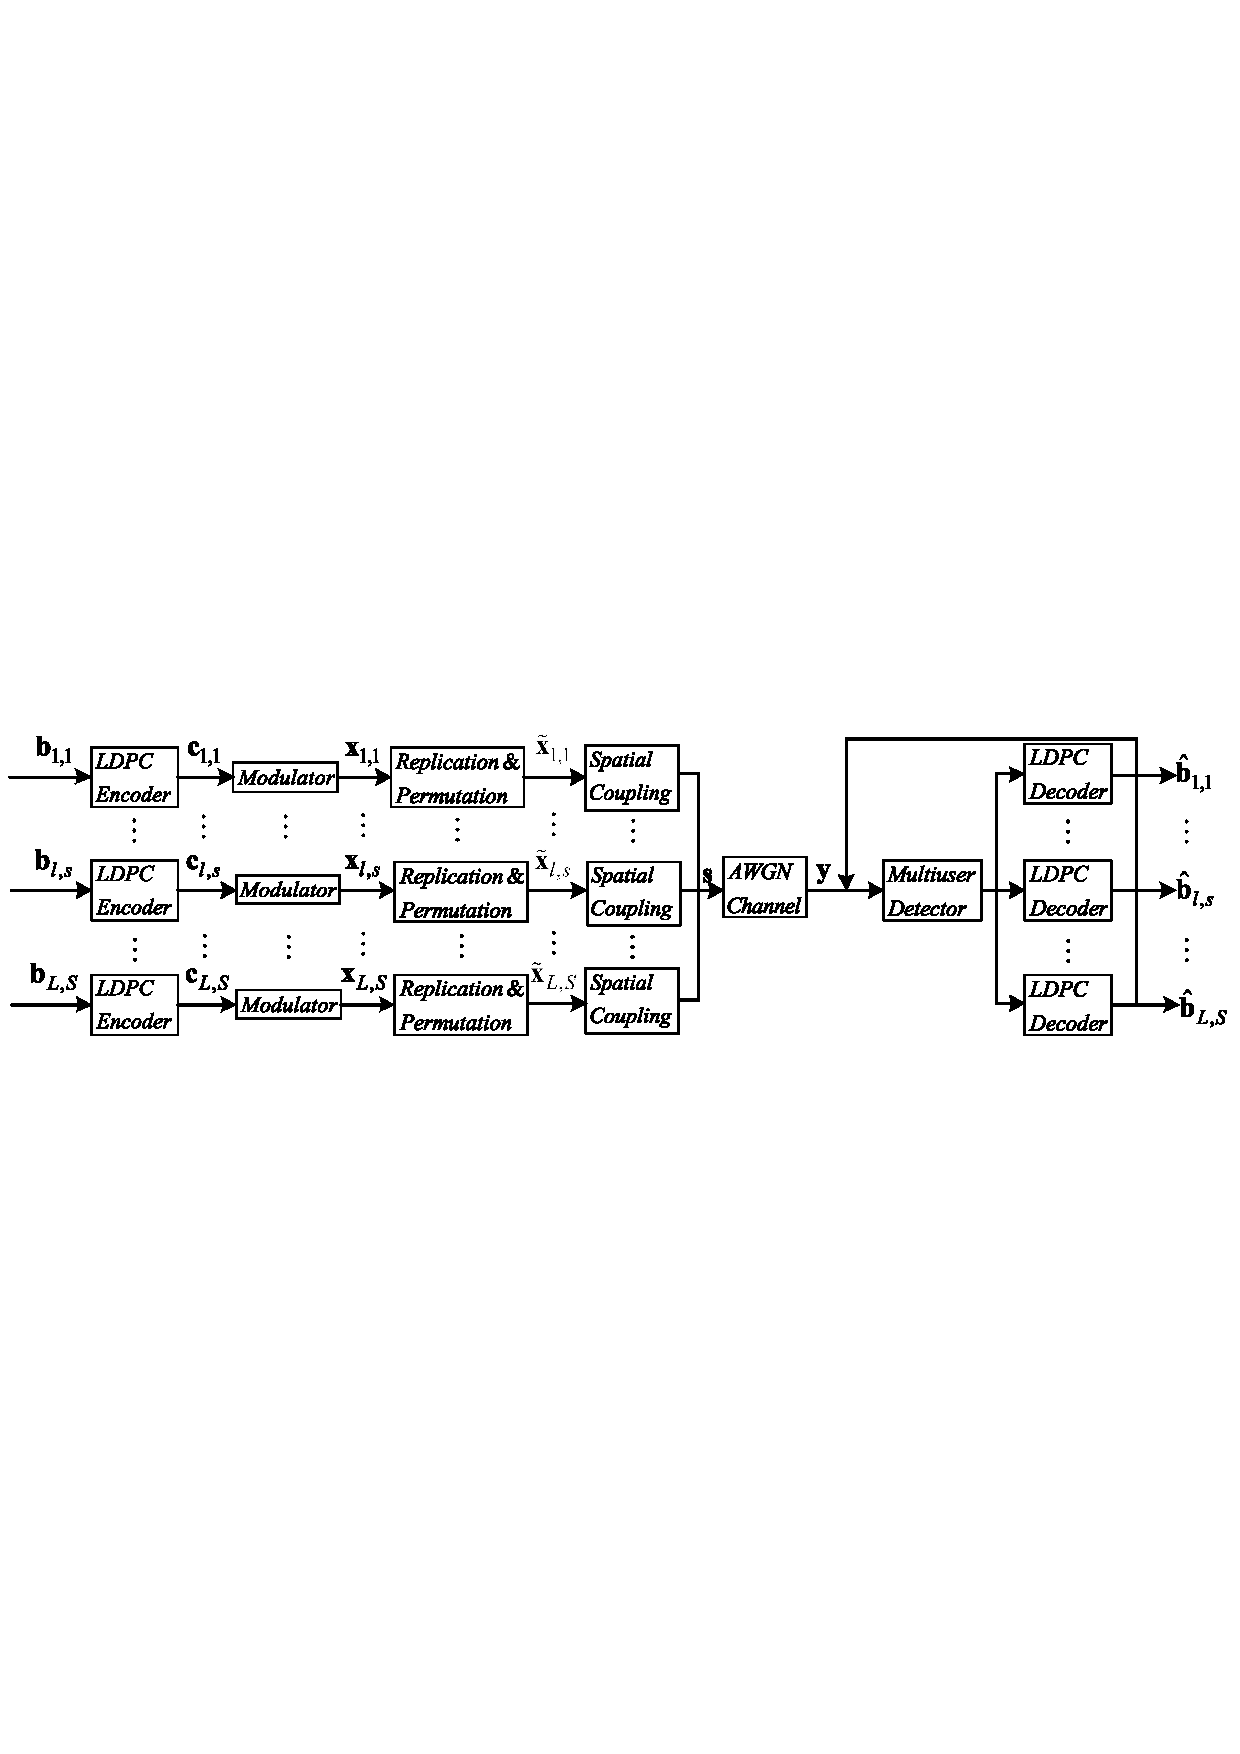
\includegraphics[scale=0.75]{1.pdf}}
  \caption{The system model of spatial coupling multiuser superposition transmission with $L$ users and $S$ data streams per user.}\label{fig.1}
    \vspace{-2em}
\end{figure*}
The system model of spatially coupled multiuser superposition transmission in this paper is shown in Fig. 1. We make assumptions that all users have the same numbers of data streams and packages and each data stream is equal-power and independent. To simplify the description, we take ${{\bf{b}}_{l,s}}$ as an example, which represents the $s$-th data stream of user $l$, $l \in \left\{ {1, \cdots ,L} \right\},s \in \left\{ {1, \cdots ,S} \right\}$, and $L$ and $S$ denote the number of user and the number of data streams per user, respectively. At the transmitter, binary information sequence ${{\bf{b}}_{l,s}} = {\left[ {{{\bf{b}}^T}_{l,s,1},{{\bf{b}}^T}_{l,s,2}, \cdots ,{{\bf{b}}^T}_{l,s,P}} \right]^T}$ in $P$ packages is encoded by LDPC encoders with code rate $R = {K \mathord{\left/
 {\vphantom {K N}} \right.
 \kern-\nulldelimiterspace} N}$, where sequence ${{\bf{b}}_{l,s,p}} = {\left[ {{b_{l,s,p,1}},{b_{l,s,p,2}}, \cdots ,{b_{l,s,p,K}}} \right]^T}$, $p \in \left\{ {1,2, \cdots ,P} \right\}$, $K$ is the length of source information in a package and $N$ is the length of the corresponding encoded codeword. In the modulator, the encoded data stream ${{\bf{c}}_{l,s}}$ is modulated with constellation rotation. The output of the modulator is denoted by sequence ${{\bf{x}}_{l,s}} = {\left[ {{{\bf{x}}^T}_{l,s,1},{{\bf{x}}^T}_{l,s,2}, \ldots ,{{\bf{x}}^T}_{l,s,P}} \right]^T}$, where ${{\bf{x}}_{l,s,p}} = {\left[ {{x_{l,s,p,1}},{x_{l,s,p,2}}, \cdots ,{x_{l,s,p,N}}} \right]^T}$. Then each package of ${{\bf{x}}_{l,s}}$ is replicated $M$ times and permuted with different interleavers, which produces signal ${{\bf{\tilde x}}_{l,s}}$ composed of $\left\{ {{\bf{\tilde x}}_{l,s,1}^1, \cdots ,{\bf{\tilde x}}_{l,s,1}^M, \cdots ,{\bf{\tilde x}}_{l,s,P}^1, \cdots ,{\bf{\tilde x}}_{l,s,P}^M} \right\}$. ${{\bf{\tilde x}}_{l,s}}$ is superimposed on other data streams to generate the signal ${\bf{s}}$ when spatial coupling. We define the system described above as a $\left( {L,S,P,M} \right)$-multiuser spatial coupling structure.

\begin{figure}[h!]
\vspace{-0.5em}
\setlength{\abovecaptionskip}{0.cm}
\setlength{\belowcaptionskip}{-0.cm}
  \centering{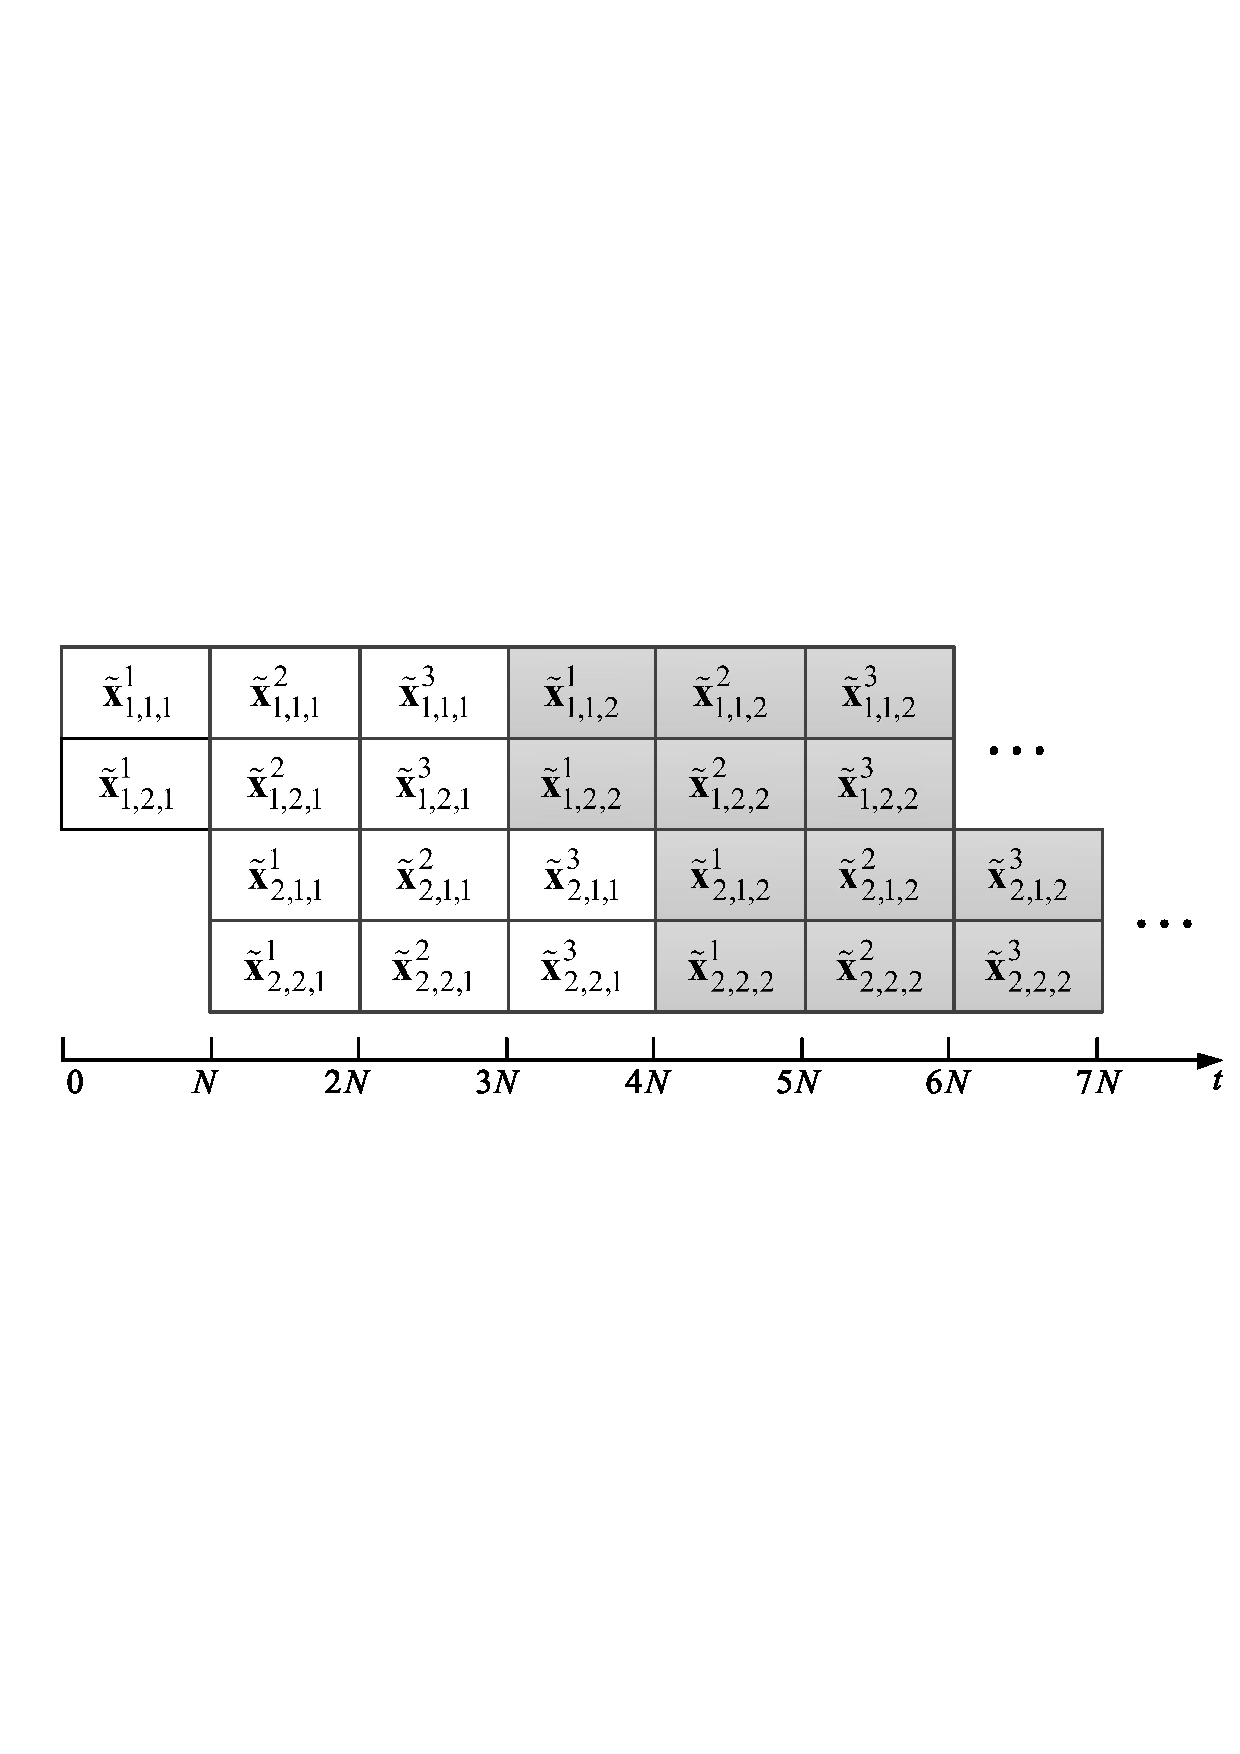
\includegraphics[scale=0.43]{2.pdf}}
  \caption{Coupling of modulated data streams with time offset $N$ in a $\left( {2,2,P,3} \right)$-multiuser spatial coupling structure.}\label{fig.2}
    \vspace{-1em}
\end{figure}
Without loss of generality, we consider the $\left( {2,2,P,3} \right)$-multiuser spatial coupling structure. The spatial coupling procedure is represented in Fig. \ref{fig.2}, where each row is a data stream of a user and the packages are transmitted one after another. The block ${\bf{\tilde x}}_{l,s,p}^m$ can be denoted as ${\bf{\tilde x}}_{l,s,p}^m = {\bm{\pi }}_{l,s,p}^m{{\bf{x}}_{l,s,p}}$, where ${\bm{\pi }}_{l,s,p}^m$ is the corresponding interleaver. At time $t = 0$, two data streams of the first user start to transmit. The signal transmitted adds two data streams of the other user after $N$ bit intervals in order.
\begin{equation}
\resizebox{1\hsize}{!}{
$\bf{H} = \left[ {\begin{array}{*{20}{c}}
{{\bm{\pi }}_{1,1,1}^1}& \cdots &{{\bm{\pi }}_{1,1,1}^M}&{ \cdots  \cdots }&{{\bm{\pi }}_{1,1,P}^1}& \cdots &{{\bm{\pi }}_{1,1,P}^M}&{}&{}&{}\\
{{\bm{\pi }}_{1,2,1}^1}& \cdots &{{\bm{\pi }}_{1,2,1}^M}&{ \cdots  \cdots }&{{\bm{\pi }}_{1,2,P}^1}& \cdots &{{\bm{\pi }}_{1,2,P}^M}&{}&{}&{}\\
 \vdots & \cdots & \vdots &{ \cdots  \cdots }& \vdots & \cdots &\vdots&{}&{}&{}\\
{{\bm{\pi }}_{1,S,1}^1}& \cdots &{{\bm{\pi }}_{1,S,1}^M}&{ \cdots  \cdots }&{{\bm{\pi }}_{1,S,P}^1}& \cdots &{{\bm{\pi }}_{1,S,P}^M}&{}&{}&{}\\
{}&{{\bm{\pi }}_{2,1,1}^1}& \cdots &{{\bm{\pi }}_{2,1,1}^M}&{ \cdots  \cdots }&{{\bm{\pi }}_{2,1,P}^1}& \cdots &{{\bm{\pi }}_{2,1,P}^M}&{}&{}\\
{}&{{\bm{\pi }}_{2,2,1}^1}& \cdots &{{\bm{\pi }}_{2,2,1}^M}&{ \cdots  \cdots }&{{\bm{\pi }}_{2,2,P}^1}& \cdots &{{\bm{\pi }}_{2,2,P}^M}&{}&{}\\
{}& \vdots & \cdots & \vdots &{ \cdots  \cdots }& \vdots & \cdots & \vdots &{}&{}\\
{}&{{\bm{\pi }}_{2,S,1}^1}& \cdots &{{\bm{\pi }}_{2,S,1}^M}&{ \cdots  \cdots }&{{\bm{\pi }}_{2,S,P}^1}& \cdots &{{\bm{\pi }}_{2,S,P}^M}&{}&{}\\
{}&{}& \ddots & \vdots & \cdots & \vdots & \cdots & \vdots &{}&{}\\
{}&{}&{}&{{\bm{\pi }}_{L,1,1}^1}& \cdots &{{\bm{\pi }}_{L,1,1}^M}&{ \cdots  \cdots }&{{\bm{\pi }}_{L,1,P}^1}& \cdots &{{\bm{\pi }}_{L,1,P}^M}\\
{}&{}&{}&{{\bm{\pi }}_{L,2,1}^1}& \cdots &{{\bm{\pi }}_{L,2,1}^M}&{ \cdots  \cdots }&{{\bm{\pi }}_{L,2,P}^1}& \cdots &{{\bm{\pi }}_{L,2,P}^M}\\
{}&{}&{}& \vdots & \cdots & \vdots &{ \cdots  \cdots }& \vdots & \cdots & \vdots \\
{}&{}&{}&{{\bm{\pi }}_{L,S,1}^1}& \cdots &{{\bm{\pi }}_{L,S,1}^M}&{ \cdots  \cdots }&{{\bm{\pi }}_{L,S,P}^1}& \cdots &{{\bm{\pi }}_{L,S,P}^M}
\end{array}} \right]$
}\label{1}
\end{equation}

We can also use spatial coupling matrix $\bf{H}$ to describe the above procedure. The construction of $\bf{H}$ is shown in (\ref{1}), where ${\bm{\pi }}_{l,s,p}^m$ is the permutation matrix of an $N  \times N $ unit matrix. Therefore, the signal $\bf{s}$ can be described as $\bf{s} = {\bf{H}^T}\bf{x}$, where ${\bf{x}} = {\left[ {{{\bf{x}}^T}_{1,1,1}, \cdots ,{{\bf{x}}^T}_{1,1,P}, \cdots ,{{\bf{x}}^T}_{L,S,1}, \cdots ,{{\bf{x}}^T}_{L,S,P}} \right]^T}$.
The total load in the system we proposed is shown in (2), which is actually the ratio between rows and columns of ${\bf{H}}$.
\begin{equation}
Load = \frac{{LSPN}}{{(PM + L - 1)N}} = \frac{{LSP}}{{PM + L - 1}}\label{2}.
\end{equation}

Considering the signal ${\bf{s}}$ is transmitted through the AWGN channel, the received signal ${\bf{y}}$ can be represented as
\begin{equation}
{\bf{y}} = \lambda {\bf{s}} + {\bf{n}}\label{3},
\end{equation}
where $\lambda $ is the power normalization coefficient, ${\bf{n}}$ is the complex AWGN with zero mean and ${{{\sigma ^2}} \mathord{\left/
 {\vphantom {{{\sigma ^2}} 2}} \right.
 \kern-\nulldelimiterspace} 2}$ variance for each dimension.

At the receiver, iterative detection and decoding based on message passing algorithm (MPA) is performed. Inner the spatial coupling structure, the extrinsic messages are iteratively exchanged along edges between channel nodes and variable nodes. For the iteration between detector and decoders, which is called outer iteration, the output of the detector is transmitted to the decoders, the outputs of the decoders is used as the input of the detector for the next iteration. Note that each package of a data stream is encoded and decoded individually and the maximum number of the outer iteration is defined as ${I_{\max }}$.
\section{CONSTELLATION ROTATION IN SPATIAL COUPLING}
\subsection{Constellation rotation}
For each data stream, the principle of constellation rotation is illustrated in Fig. \ref{fig.3}, where the modulated signal is constructed by anticlockwise rotating the standard modulation with a certain angle $\theta $, ${\theta} \in \left[ {0,180} \right)$.
\begin{figure}[h!]
\setlength{\abovecaptionskip}{0.cm}
\setlength{\belowcaptionskip}{-0.cm}
  \centering{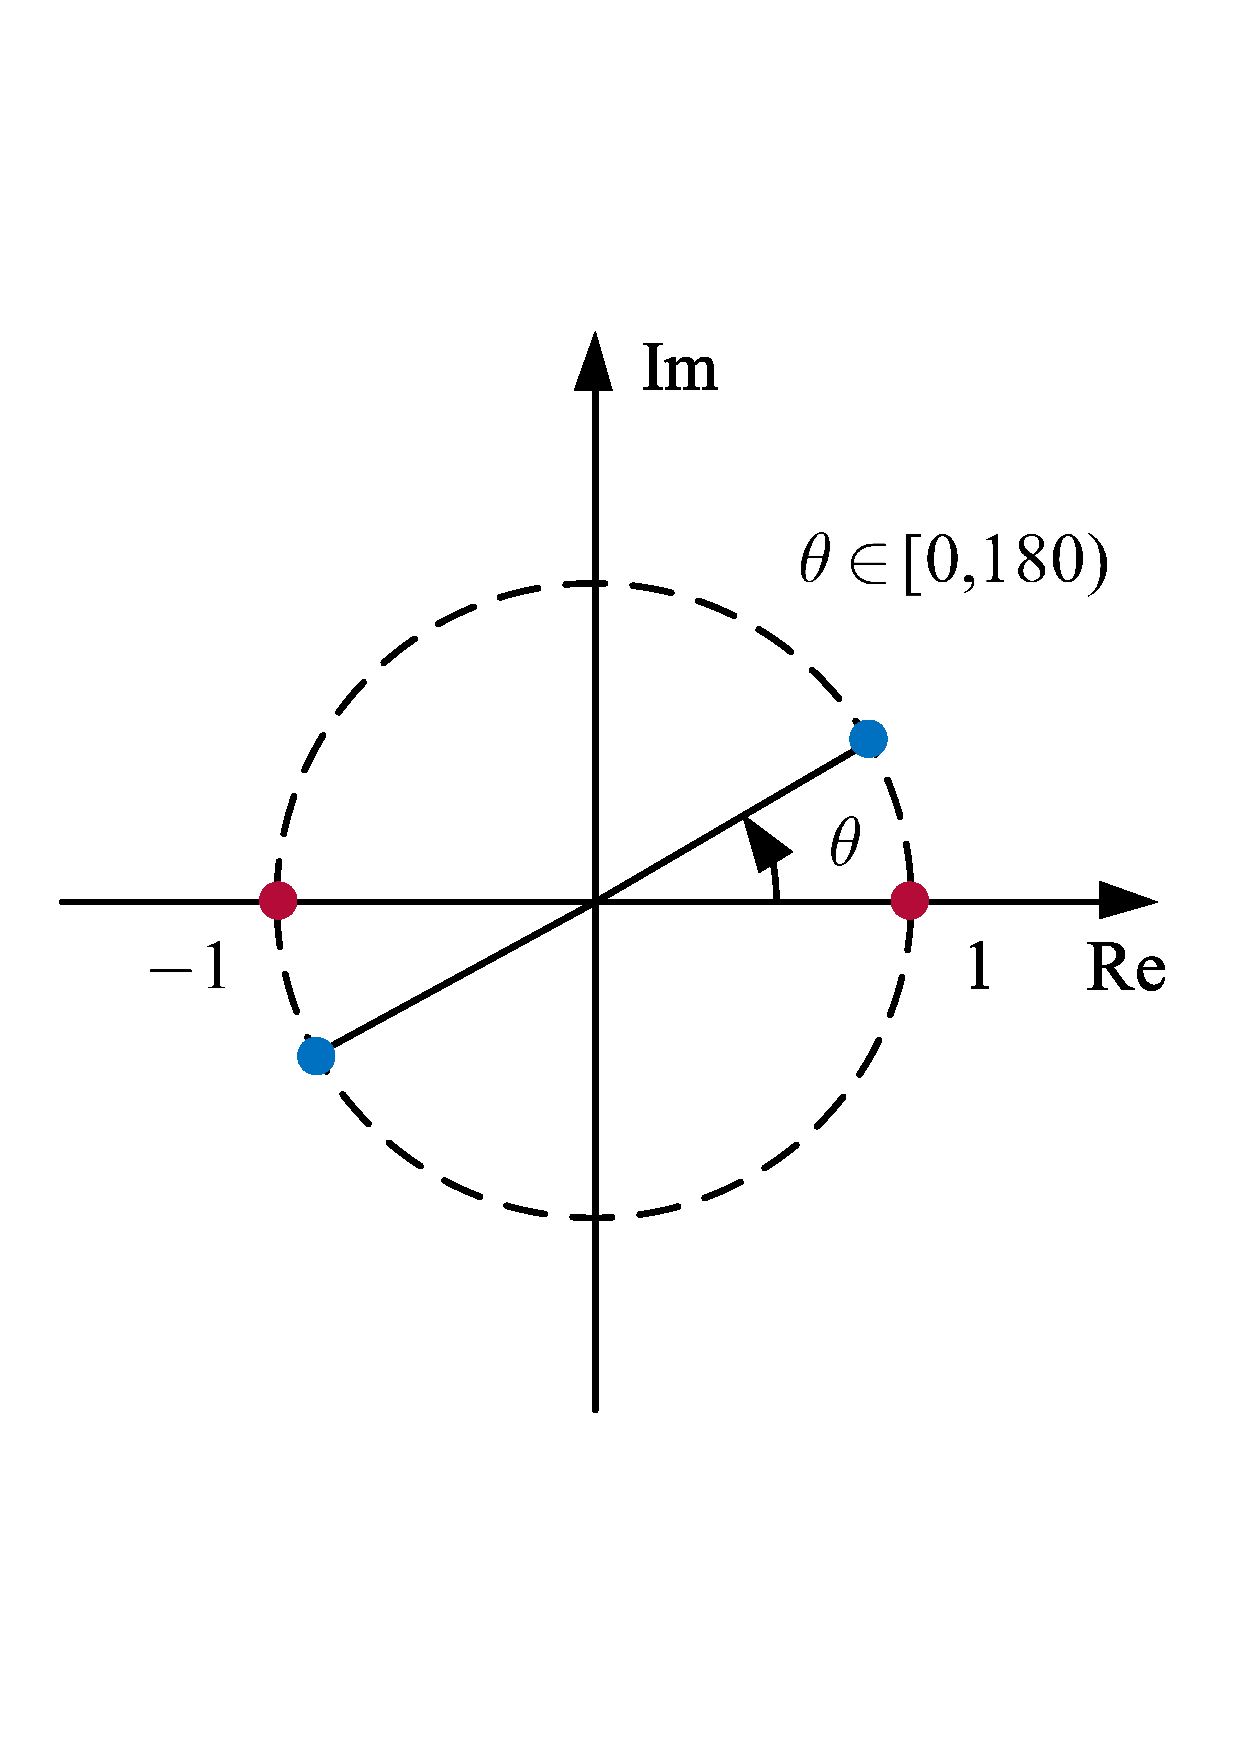
\includegraphics[scale=0.20]{3.pdf}}
  \caption{The constellation rotation of each data stream.}
    \vspace{-1em}\label{fig.3}
\end{figure}

Assuming ${\bf{x}}{'_{l,s}}$ denotes the BPSK modulated signal of ${{\bf{c}}_{l,s}}$, ${\bf{x}}{'_{l,s}} = {\left[ {{\bf{x}}{'^T}_{l,s,1},{\bf{x}}{'^T}_{l,s,2}, \cdots ,{\bf{x}}{'^T}_{l,s,P}} \right]^T}$. Then ${\bf{x}}{'_{l,s}}$ is rotated with angle ${{\theta} _{l,s}}$, and ${{\bf{x}}_{l,s}}$ can be described as
\begin{equation}
{{\bf{x}}_{l,s}} = {e^{i{{\theta} _{l,s}}}}{\bf{x}}{'_{l,s}}\label{4}.
\end {equation}

\subsection{Spatially coupling based on constellation rotation}
To our knowledge, there exists inevitable interference when different signals are superimposed in spatially coupled multiuser superposition transmission. Therefore, we introduce the constellation rotation to make a further distinction between the superimposed signals.

(\uppercase\expandafter{\romannumeral1}) We deal with the interference between different data streams of each user by rotating them with different angles, and there is no difference between users. It diversifies the constellation of the coupled signal ${\bf{s}}$ and contributes to improving the performance of the system theoretically.

(\uppercase\expandafter{\romannumeral2}) To distinguish the interference between different users, we use different angles to modulate all different data streams, which expands the diversity at the cost of increasing the implementation complexity. Experimental results show that the increase in complexity is negligible when compared to the improvement of performance.
\begin{figure}[h!]
\setlength{\abovecaptionskip}{0.cm}
\setlength{\belowcaptionskip}{-0.cm}
  \centering{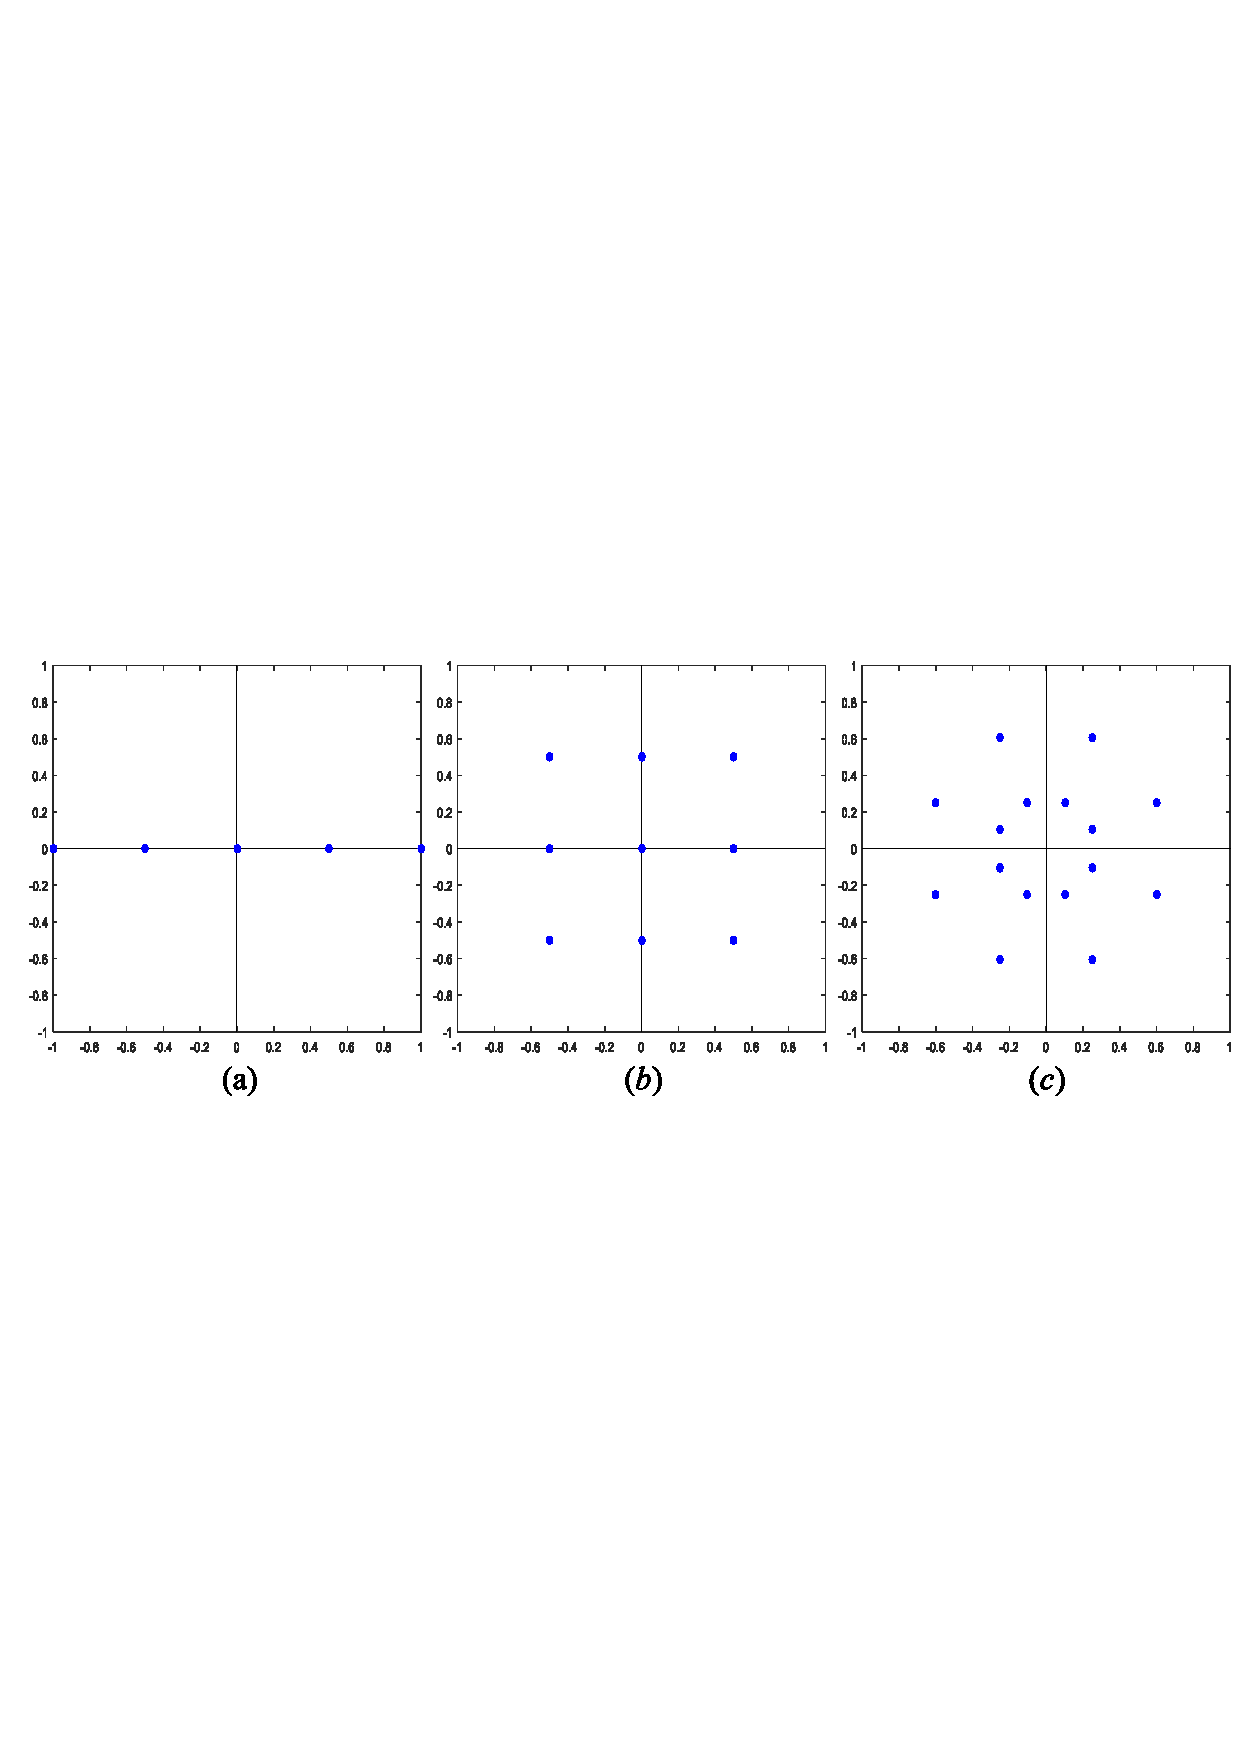
\includegraphics[scale=0.42]{4.pdf}}
  \caption{The constellations of coupled signal ${\bf{s}}$ in $(2,2,P,S)$-multiuser spatial coupling system. Rotation angle sets from left to right are $\left( {0,0,0,0} \right)$, $\left( {0,90,0,90} \right)$ and $\left( {0,30,60,90} \right)$, respectively.}\label{fig.4}
    \vspace{-1em}
\end{figure}

We take the $(2,2,P,S)$-multiuser spatial coupling system as observation, and the constellations of ${\bf{s}}$ with different rotation angle sets are shown in Fig. \ref{fig.4}. As can be seen from the figure, the constellation of ${\bf{s}}$ may contain $16$ points when all data streams are modulated with different angles. There exists constellation overlapping when different users use the same rotation rule, we also call this phenomenon constellation aliasing. Nonetheless, both of them obtain higher diversity in constellation compared with the system without any constellation rotation.

When considering constellation, we naturally come up with the minimum Euclidean distance which reflects the interference between constellation points. The minimum Euclidean distance decreases when the diversity of the constellation increases. Therefore, it is necessary to make a trade off between constellation aliasing and interference and search for the optimal rotation angles.
\subsection{Rotation angle optimization}
The optimization of rotation angles can be carried out by maximizing AMI between the input ${\bf{S}}$ and the output ${\bf{Y}}$. The maximum AMI represents the maximum amount of information about ${\bf{S}}$ that can be conveyed through the channel. Assuming the constellation point set of ${\bf{S}}$ is denoted by $\left\{ {{\hat s_t}} \right\},t \in \left\{ {1,2, \cdots ,T = {2^{LS}}} \right\}$, ${\hat s_t} = {a_t} + i{b_t}$, and $y$ represents the element in ${\bf{Y}}$, $y = u + iv$. The channel transition probability is given as
\begin{equation}
\begin{aligned}
p(y|{\hat s_t}) &= \int\int{\frac{1}{{\pi {N_0}}}{e^{ - \;\frac{{{{\left( {u - {a_t}} \right)}^2} + {{\left( {v - {b_t}} \right)}^2}}}{{{N_0}}}}}dudv} \\
&= \int\int\frac{1}{{\pi {N_0}}}{e^{ - \;\frac{{{{\left| {y - {\hat s_t}} \right|}^2}}}{{{N_0}}}}}dudv\label{5},
\end{aligned}
\end{equation}
where $N_0$ is the noise power spectral density. In order to facilitate the calculation, we assume that $N_0=1$. The computational formula of MI is derived as
\begin{equation}
\begin{aligned}
I\left( {\bf{S};\bf{Y}} \right) = \sum\limits_{t = 1}^T {p\left( {{\hat s_t}} \right)} \int \int p\left( {y|{\hat s_t}} \right)\log \frac{{p\left( {y|{\hat s_t}} \right)}}{{\sum\nolimits_{t = 1}^T {p\left( {{\hat s_t}} \right)p\left( {y|{\hat s_t}} \right)} }}dudv\label{6}.
\end{aligned}
\end{equation}
As $\hat s_t$ occurs with equal probability, we combine (\ref{5}) and (\ref{6}), and get
\begin{equation}
\begin{aligned}
&I\left( {\bf{S};\bf{Y}} \right) = \log T - \\
&\frac{1}{T}\sum\limits_{t = 1}^T {\int\int\frac{1}{{\pi {N_0}}}{e^{ - \;\frac{{{{\left| {y - {\hat s_t}} \right|}^2}}}{{{N_0}}}}}\log \sum\limits_{t' = 1}^T {{e^{ - \;\frac{{{{\left| {y - {\hat s_{t'}}} \right|}^2} + {{\left| {y - {\hat s_t}} \right|}^2}}}{{{N_0}}}}}} dudv}\label{7}.
\end{aligned}
\end{equation}

In our scheme, we traverse all sets of rotation angles when the total number of data streams $LS$ is determined, we use the symmetry to reduce the complexity and stop the traversal the moment the AMI reach its maximum.
\subsection{Iterative detection and decoding}
In this section, we describe the process of iterative detection and decoding scheme in detail. During the detection, the LLRs are used as the extrinsic information and passed between nodes given in Fig. \ref{fig.5}. The received message of one node along one edge is not allowed to update the message sent from the same edge.

\begin{figure}[h!]
\setlength{\abovecaptionskip}{0.cm}
\setlength{\belowcaptionskip}{-0.cm}
  \centering{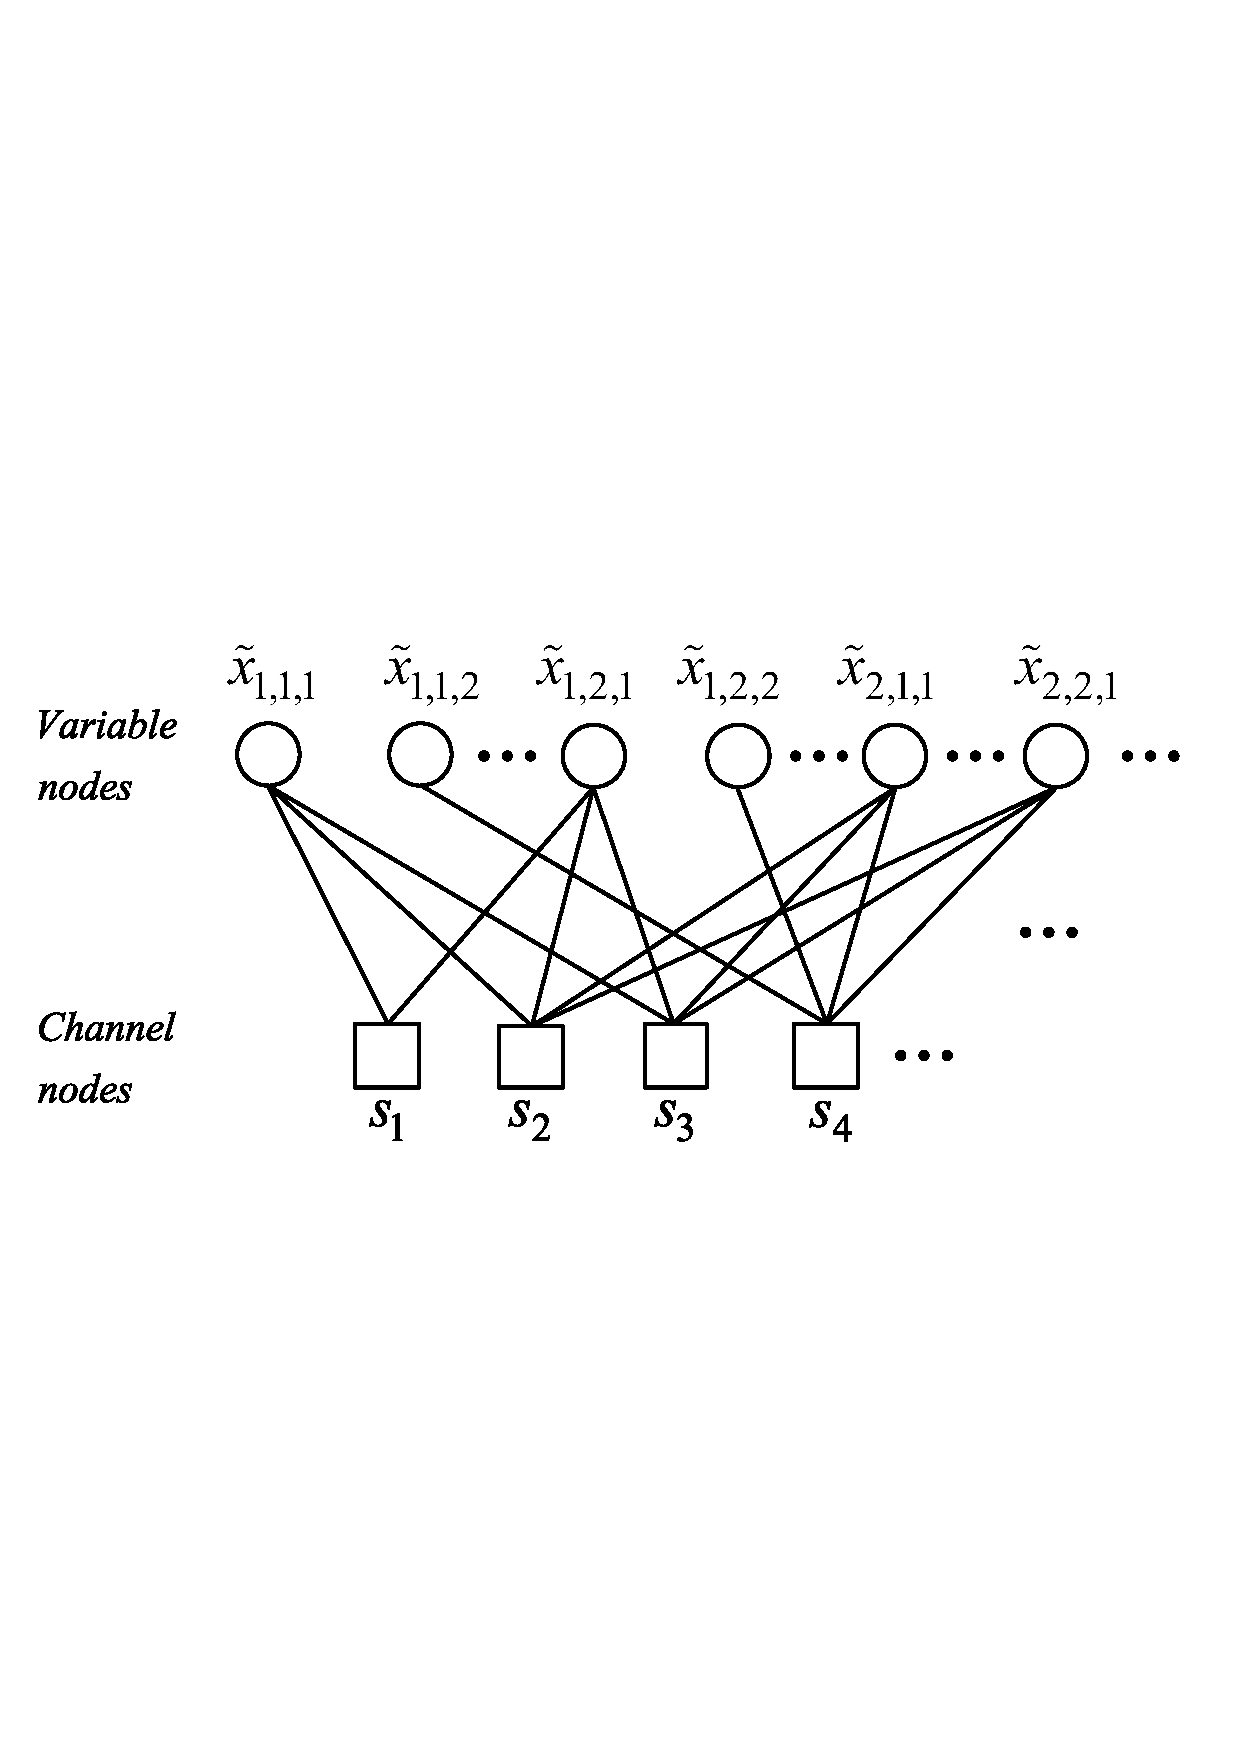
\includegraphics[scale=0.37]{5.pdf}}
  \caption{Factor graph representation of spatial coupling multiple access system, where circles represent variable nodes corresponding to the data blocks in Fig. \ref{fig.2}, channel nodes are coupled data and denoted by squares.}\label{fig.5}
    \vspace{-1em}
\end{figure}
Take the edge between variable node ${\tilde {x}_{l,s,p}}$ and channel node ${s_t}$ as observation. Set $\xi (l,s,p)\backslash t$ as the index collection of channel nodes connected with variable node ${\tilde {x}_{l,s,p}}$ and set $\zeta t\backslash (l,s,p)$ as the index collection of variable nodes connected with channel nodes ${s_t}$. Symbol ${l_{{{\tilde {x}}_{l,s,p}} \to {s_t}}}$ and ${l_{{s_t} \to {{\tilde {x}}_{l,s,p}}}}$ represent the message sent from ${\tilde {x}_{l,s,p}}$ and ${s_t}$, respectively. We initialize ${l_{{{\tilde {x}}_{l,s,p}} \to {s_t}}}$ as follows
\begin{equation}
{l_{{{\tilde x}_{l,s,p}} \to {s_t}}} = \log {\rm{ }}\frac{{p({{\tilde x}_{l,s,p}} =  + {e^{i{\theta _{l,s}}}})}}{{p({{\tilde x}_{l,s,p}} =  - {e^{i{\theta _{l,s}}}})}}\label{8}.
\end{equation}
The message updated during the iteration can be write as
\begin{equation}
\begin{aligned}
{l_{{{\tilde {x}}_{l,s,p}} \to {s_t}}} = \sum\limits_{_{t' \in \xi (l,s,p)\backslash t}} {{l_{{s_{t'}} \to {{\tilde {x}}_{l,s,p}}}}}\label{9},
\end{aligned}
\end{equation}
\begin{equation}
\begin{aligned}
{l_{{s_t} \to {{\tilde {x}}_{l,s,p}}}}\;\;\;{\kern 1pt}  = \;\;\;{\kern 1pt} \log \frac{{p({{\tilde {x}}_{l,s,p}} =  + {e^{i{\theta _{l,s}}}}|{s_t},{{\bf{\tilde x}}^{[t]}}\backslash {{\tilde {x}}_{l,s,p}})}}{{p({{\tilde {x}}_{l,s,p}} =  - {e^{i{\theta _{l,s}}}}|{s_t},{{\bf{\tilde x}}^{[t]}}\backslash {{\tilde {x}}_{l,s,p}})}} \\
= \log \frac{{p({s_t}|{{\bf{\tilde x}}^{[t]}},{{\tilde {x}}_{l,s,p}} =  + {e^{i{\theta _{l,s}}}})p({{\bf{\tilde x}}^{[t]}}|{{\tilde {x}}_{l,s,p}} =  + {e^{i{\theta _{l,s}}}})}}{{p({s_t}|{{\bf{\tilde x}}^{[t]}},{{\tilde {x}}_{l,s,p}} =  - {e^{i{\theta _{l,s}}}})p({{\bf{\tilde x}}^{[t]}}|{{\tilde {x}}_{l,s,p}} =  - {e^{i{\theta _{l,s}}}})}}\label{10},
\end{aligned}
\end{equation}
where ${{\bf{\tilde {\bf{x}}}}^{[t]}}$ denotes the set containing all signals superimposed on the coupled signal ${{s_t}}$. Equation (\ref{10}) is derived by using Bayes' rule listed below
\begin{equation}
\begin{aligned}
p(x|y) = \frac{{p(y|x)p(x)}}{{p(y)}}\propto p(y|x)p(x)\label{11}.
\end{aligned}
\end{equation}
The conditional probability density function (pdf) of the coupled signal ${{s_t}}$ and the set ${{\bf{\tilde x}}^{[t]}}$ are given separately as
\begin{equation}
p\left( {{s_t}|{{\bf{\tilde x}}^{[t]}}} \right) = \frac{1}{{\sqrt {2\pi \sigma } }}\exp \left( { - {\mkern 1mu} \frac{1}{{2{\sigma ^2}}}{{\left\| {{s_t} - {{\bf{h}}^{[t]T}}{{\bf{\tilde x}}^{[t]}}} \right\|}^2}} \right)\label{12},
\end{equation}
\begin{equation}
\begin{aligned}
p\left( {{{\bf{\tilde x}}^{[t]}}|{{\tilde {x}}_{l,s,p}}} \right) = {\prod _{(l',s',p') \in \zeta t\backslash (l,s,p)}}p({\tilde {x}_{l',s',p'}})\label{13},
\end{aligned}
\end{equation}
where ${{\bf{h}}^{[t]}}$ is the normalized coefficient vector of ${{\bf{\tilde x}}^{[t]}}$. The symbol $\left\| {} \right\|$ is modulus operation and a priori probability of ${\tilde {x}_{l',s',p'}}$ is written as
\begin{equation}
p({\tilde {x}_{l',s',p'}}) = \exp \left( {\frac{{{{\tilde {x}}_{l',s',p'}}}}{2}{l_{{{\tilde {x}}_{l',s',p'}} \to {s_t}}}} \right)\label{14}.
\end{equation}

\begin{figure*}[ht]
\begin{equation}
\begin{aligned}
{l_{{s_t} \to {{\tilde {x}}_{l,s,p}}}} = \mathop {{{\max }^ \star }}\limits_{\begin{array}{*{20}{c}}
{\;\;\;\;\;\;{{\bf{\tilde x}}^{[t]}}\;\;\;\;\;\;}\\
{{{\tilde {x}}_{l,s,p}} =  + {e^{i{\theta _{l,s}}}}}
\end{array}} \left( {{\sum _{(l',s',p') \in \zeta t\backslash (l,s,p)}}\frac{{{{\tilde {x}}_{l,s,p}}}}{2}{l_{{{\tilde {x}}_{l,s,p}} \to {s_t}}} - \frac{1}{{2{\sigma ^2}}}{{\left\| {{s_t} - {{\bf{\bf{h}}}^{[t]T}}{{\bf{\tilde x}}^{[t]}}} \right\|}^2}} \right) \\- \mathop {{{\max }^ \star }}\limits_{\begin{array}{*{20}{c}}
{\;\;\;\;\;\;{{\bf{\tilde x}}^{[t]}}\;\;\;\;\;\;}\\
{{{\tilde {x}}_{l,s,p}} =  - {e^{i{\theta _{l,s}}}}}
\end{array}} \left( {{\sum _{(l',s',p') \in \zeta t\backslash (l,s,p)}}\frac{{{{\tilde x}_{l,s,p}}}}{2}{l_{{{\tilde {x}}_{l,s,p}} \to {s_t}}} - \frac{1}{{2{\sigma ^2}}}{{\left\| {{s_t} - {{\bf{\bf{h}}}^{[t]T}}{{\bf{\tilde x}}^{[t]}}} \right\|}^2}} \right)\label{15}.
\end{aligned}
\end{equation}
\rule{\textwidth}{0.2mm}
\vspace{-2em}
\end{figure*}
Substituting (\ref{12}), (\ref{13}) and (\ref{14}) into (\ref{10}), we get (\ref{15}) shown on the top of next page, where ${\mathop {\max }\nolimits^* }$ operation \cite{11} is defined as follows
\begin{equation}
\begin{aligned}
\mathop {\max }\nolimits^* (a,b) &= \log (\exp (a) + \exp (b)) \\&= \max(a,b) + \log(1 + \exp ( - \left| {a - b} \right|))\label{16}.
\end{aligned}
\end{equation}

We define the iterative process from the detector to the decoders as a complete iteration. The message exchanged between the detector and the decoders can be described as
\begin{equation}
\begin{aligned}
l_{out,{{\tilde {x}}_{l,s,p}}}^{DEC[i]} = l_{{{\tilde {x}}_{l,s,p}}}^{{I_{DEC}}} - l_{out,{{\tilde {x}}_{l,s,p}}}^{DET[i]}\label{17},
\end{aligned}
\end{equation}
where the symbol on the left side of the equation represents the output of the decoder in the $i$-th iteration, $i \in \left\{ {1, \cdots {I_{\max }}} \right\}$. On the right side, the subtrahend is the LLR of the decoder after ${{I_{DEC}}}$ inner iterations and is used for soft decision, the minuend denotes the output of the detector in $i$-th iteration, initialized as $0$ when $i=1$ and is updated as
\begin{equation}
\begin{aligned}
l_{out,{{\tilde {x}}_{l,s,p}}}^{DET[i]} = l_{{{\tilde {x}}_{l,s,p}}}^{{I_{DET}}} - l_{out,{{\tilde {x}}_{l,s,p}}}^{DEC[i - 1]}\label{18},
\end{aligned}
\end{equation}
where $l_{{{\tilde {x}}_{l,s,p}}}^{{I_{DET}}}$ is the total LLR received from neighbors of ${{{\tilde {x}}_{l,s,p}}}$ after ${{I_{DET}}}$ inner iterations. The symbol $l_{out,{{\tilde {x}}_{l,s,p}}}^{DEC[i - 1]}$ is the $(i - 1)-$th iterative output of the detector.

\section{SIMULATION RESULTS AND DISCUSSIONS}
In this section, we analyze the system performance using EXIT charts and BER curves. The system parameters are configured as follows. The encoding scheme considered is $(3,6)$-regular LDPC code with length $N=1800$ and rate ${1 \mathord{\left/
 {\vphantom {1 2}} \right.
 \kern-\nulldelimiterspace} 2}$.
\subsection{EXIT chart}
EXIT chart is a useful tool to track the MI at each iteration in soft-in soft-out (SISO) system, and it provides an excellent prediction on the behavior of the iteration. We use EXIT charts to evaluate the performance of the detector (or decoders) by observing whether it is conductive to increase the output mutual information ${I_E}$ when the input extrinsic information ${I_A}$ is given. We produce the EXIT curve with input mutual information and the corresponding output of the detector.

\begin{figure}[h!]
\setlength{\abovecaptionskip}{0.cm}
\setlength{\belowcaptionskip}{-0.cm}
  \centering{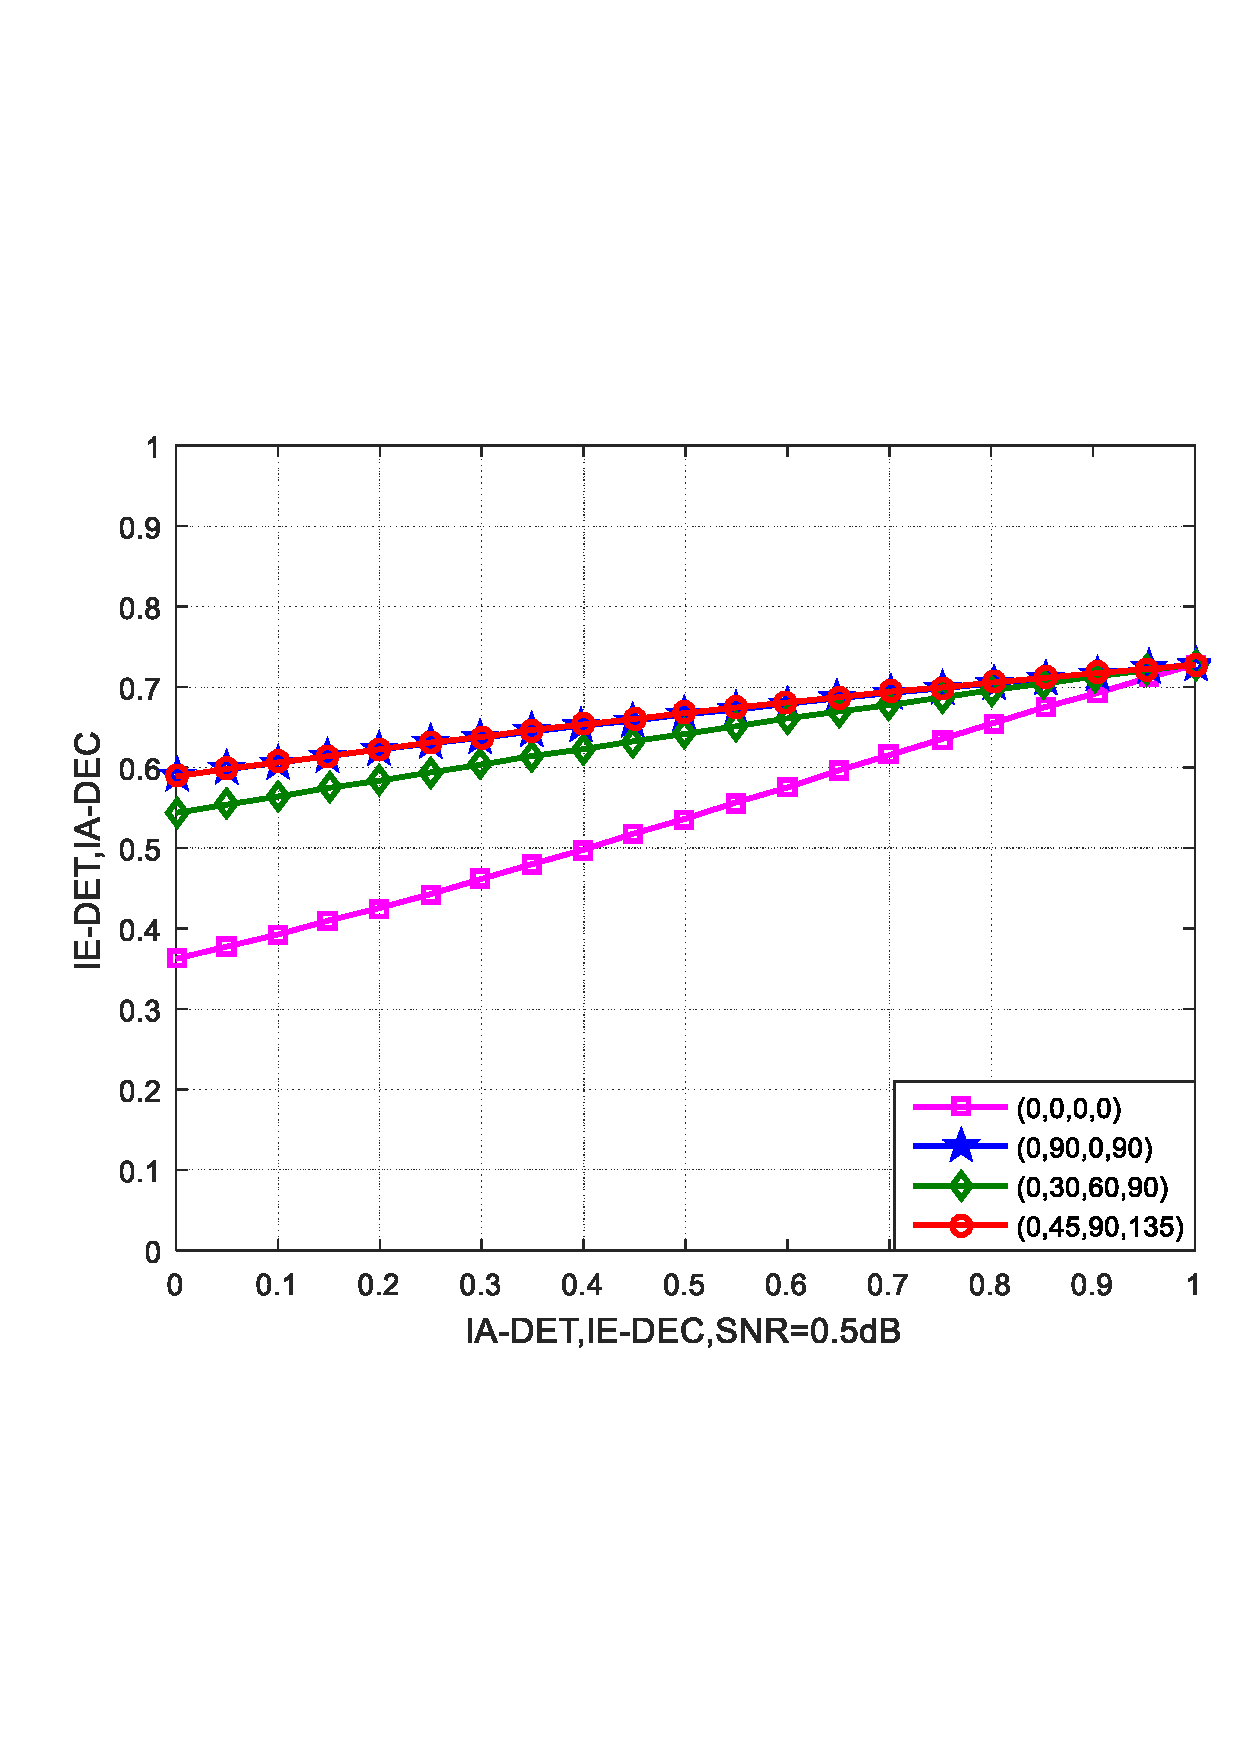
\includegraphics[scale=0.33]{6.pdf}}
  \caption{The EXIT curve of the detector with different rotation angle set in the $\left( {2,2,5,2} \right)$-multiuser spatial coupling structure with SNR = 0.5dB.}\label{fig.6}
    \vspace{-1em}
\end{figure}
\begin{figure}[h!]
\setlength{\abovecaptionskip}{0.cm}
\setlength{\belowcaptionskip}{-0.cm}
  \centering{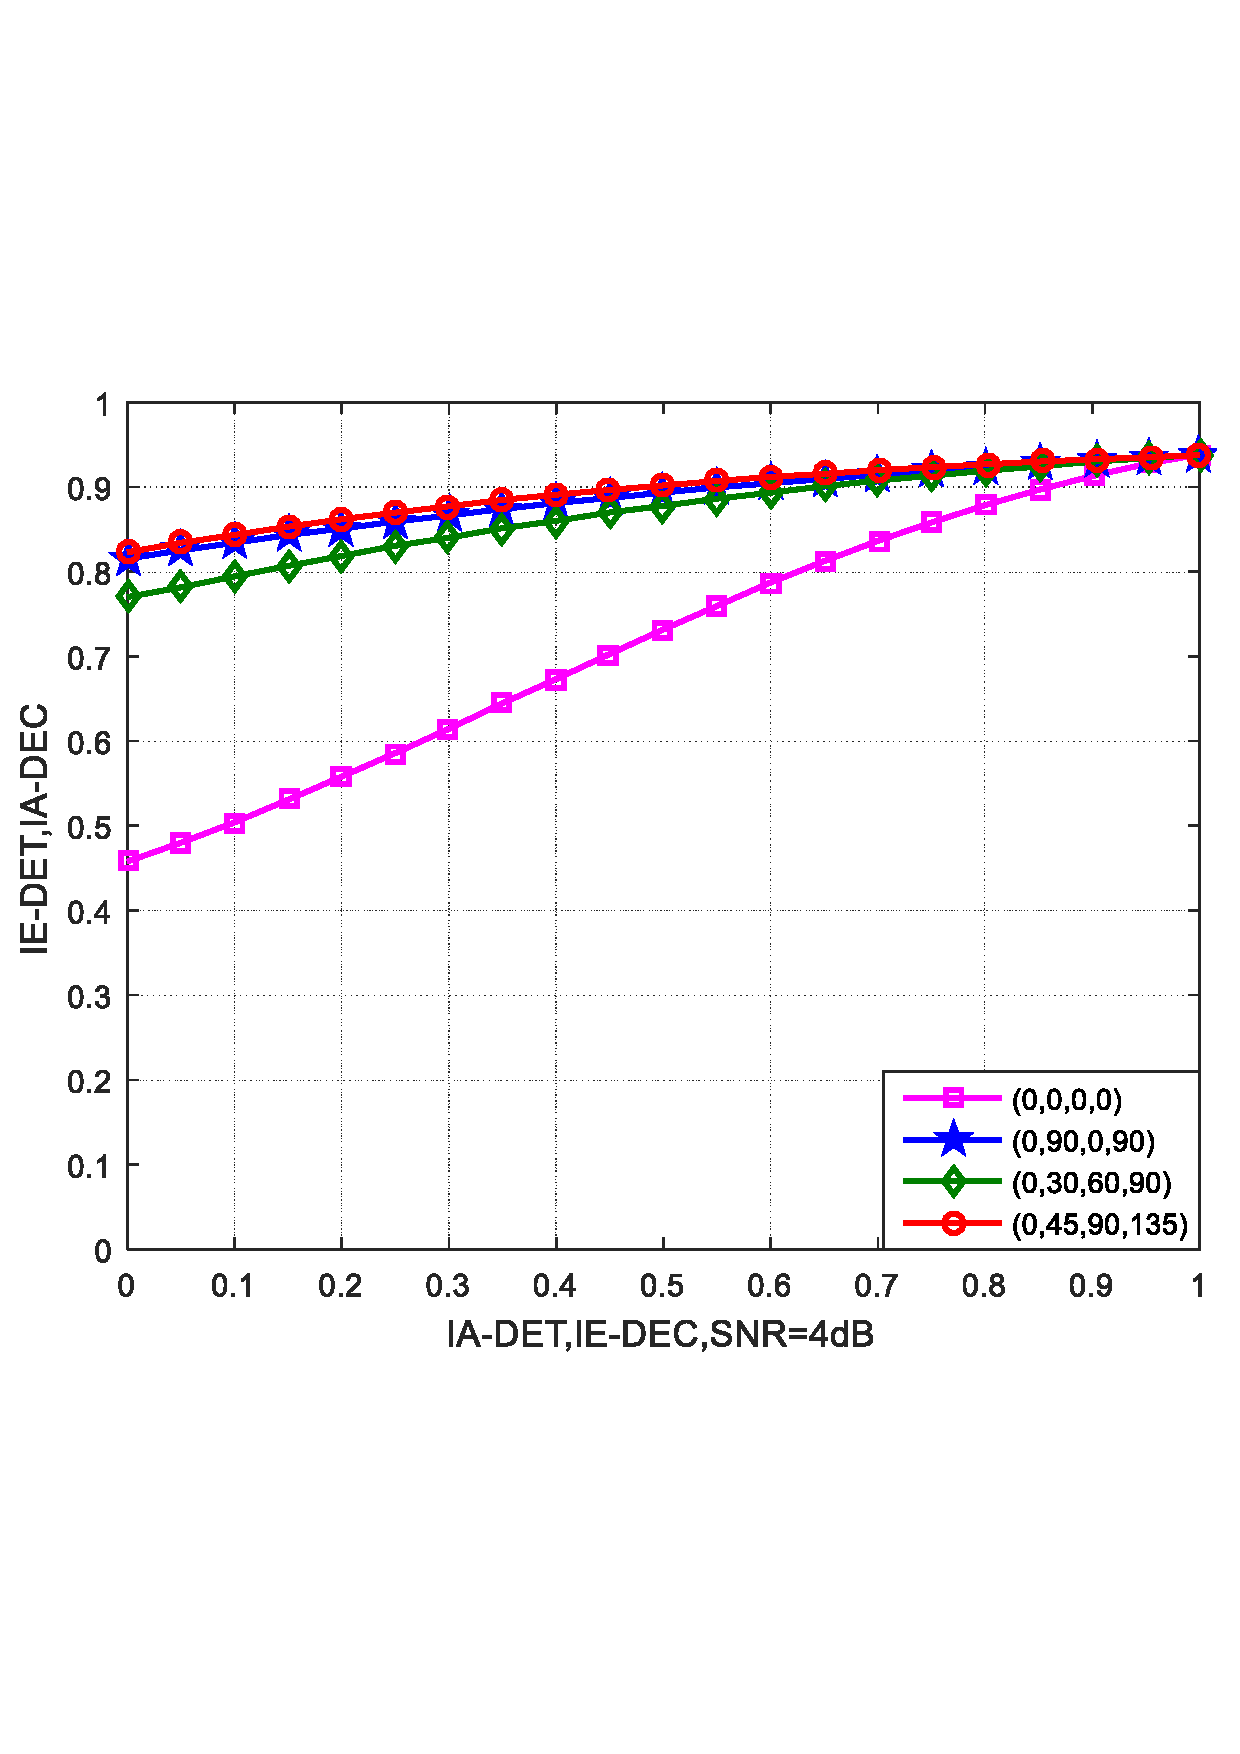
\includegraphics[scale=0.31]{7.pdf}}
  \caption{The EXIT curve of the detector with different rotation angle set in the $\left( {2,2,5,2} \right)$-multiuser spatial coupling structure with SNR = 4dB.}\label{fig.7}
    \vspace{-0.5em}
\end{figure}

We take the $(2,2,5,2)$-multiuser spatial coupling structure as an instance. There are two EXIT curves of detector with different rotation angle set over AWGN channel at SNR = 0.5dB shown in Fig. \ref{fig.6} and SNR = 4dB shown in Fig. \ref{fig.7}, respectively. According to the figures above, we reach a conclusion that constellation rotation does contribute to increase the output mutual information of the detector. When we only consider the interference between two data streams of the same user, the optimal rotation angle set is $(0,90,0,90)$, namely, two data streams of each user are orthogonal to each other. That means there exists no interference between certain user's different data streams, but the interference between the two users can not be eliminated and results in the constellation aliasing. When all data streams are taken into account, the diversity of constellation increases. In this case, the optimal rotation angle set we seek out is $(0,90,45,135)$. It can be seen that when the SNR is 0.5dB, the performance of the detector for $(0,90,45,135)$ is almost the same as that for $(0,90,0,90)$. That is to say interference plays a dominant role in the factors affecting the performance rather than diversity. On the contrary, when the SNR is 4dB, the performance of detector is better for $(0,90,45,135)$, which means diversity is the main influencing factor. Anyway, both of them perform better than the system with rotation angle sets randomly selected, such as $(0,30,60,90)$.
\subsection{BER curve}
We have demonstrated that the constellation rotation is applicable to any spatial coupling multiuser superposition transmission structure. In this subsection, we only take the $(2,2,5,2)$-multiuser spatial coupling structure and the $(3,2,6,3)$-multiuser spatial coupling structure as observations. The optimal rotation angle sets we obtain are $(0,90,45,135)$ and $(0,90,30,120,60,150)$, respectively.

\begin{figure}[h!]
\setlength{\abovecaptionskip}{0.cm}
\setlength{\belowcaptionskip}{-0.cm}
  \centering{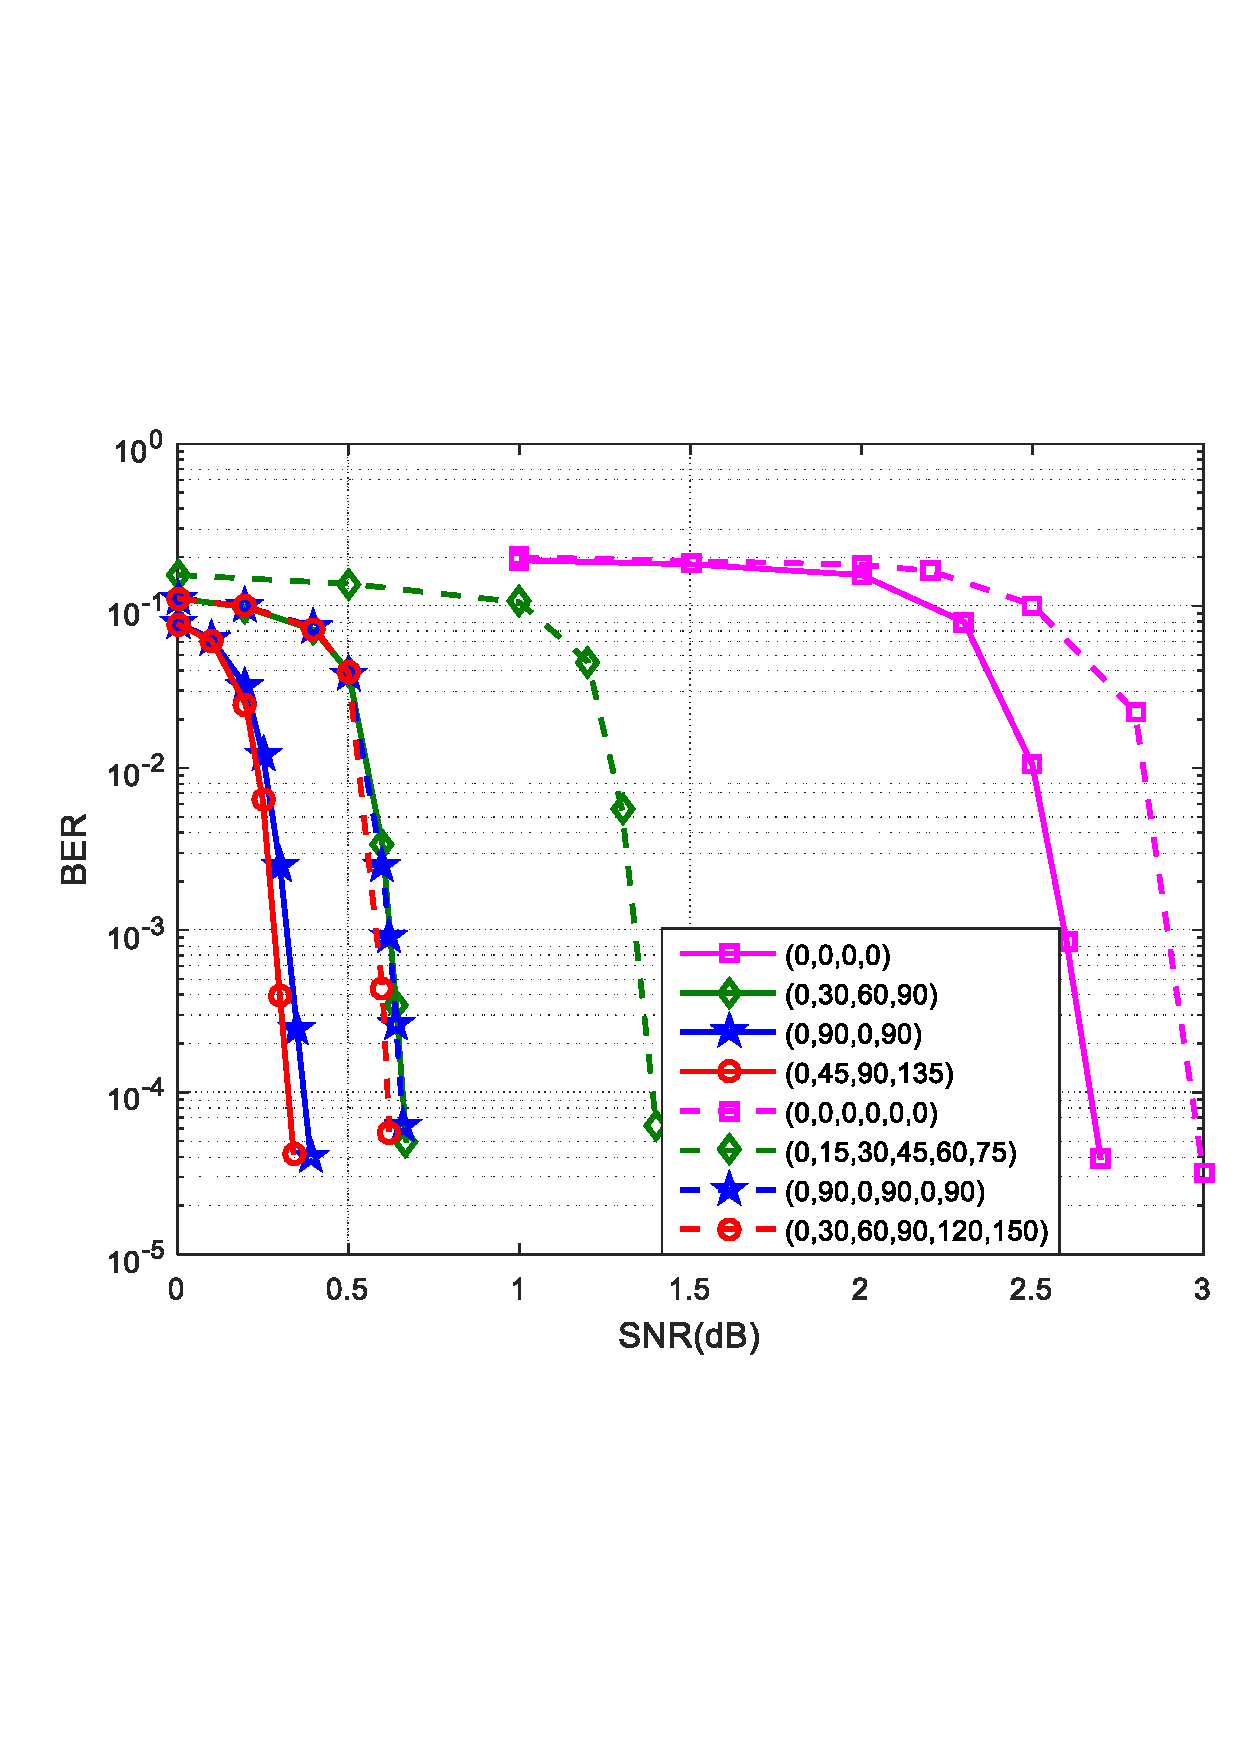
\includegraphics[scale=0.35]{8.pdf}}
  \caption{The average BER curves of different spatially coupled multiuser superposition transmission systems with different rotation angle sets.}\label{fig.8}
    \vspace{-1em}
\end{figure}
We illustrate the average BER curves of the system in Fig. \ref{fig.8}, where solid lines and dotted lines represent the systems with the structure $\left( {2,2,5,2} \right)$ and the structure $\left( {3,2,6,3} \right)$, respectively. It can be observed that the system with constellation rotation achieves the better performance indeed and the optimal rotation angle sets we have found out outperform the others in terms of BER performance, which is consistent with the analysis of EXIT charts above. In addition, the performance of the system with constellation rotation converges faster, which is beneficial to reduce the implementation complexity and the latency of the system.
\section{CONCLUSIONS}
In this paper, we have introduced constellation rotation into spatially coupled multiuser superposition transmission. We have sought out the optimal rotation angle set by maximizing the AMI. The EXIT charts and BER simulation results verify that the constellation rotation benefits to improve the system performance and reduce the implementation complexity and the latency. The system with the optimal rotation angle set performs better than the others.
% use section* for acknowledgment
%\section*{Acknowledgment}


%The authors would like to thank...





% trigger a \newpage just before the given reference
% number - used to balance the columns on the last page
% adjust value as needed - may need to be readjusted if
% the document is modified later
%\IEEEtriggeratref{8}
% The "triggered" command can be changed if desired:
%\IEEEtriggercmd{\enlargethispage{-5in}}

% references section

% can use a bibliography generated by BibTeX as a .bbl file
% BibTeX documentation can be easily obtained at:
% http://www.ctan.org/tex-archive/biblio/bibtex/contrib/doc/
% The IEEEtran BibTeX style support page is at:
% http://www.michaelshell.org/tex/ieeetran/bibtex/
%\bibliographystyle{IEEEtran}
% argument is your BibTeX string definitions and bibliography database(s)
%\bibliography{IEEEabrv,../bib/paper}
%
% <OR> manually copy in the resultant .bbl file
% set second argument of \begin to the number of references
% (used to reserve space for the reference number labels box)
\begin{thebibliography}{100}

\bibitem{1}
L. Dai, B. Wang, Y. Yuan, S. Han, C. l. I and Z. Wang, ``Non-orthogonal multiple access for 5G: solutions, challenges, opportunities, and future research trends," in IEEE Communications Magazine, vol. 53, no. 9, pp. 74-81, September 2015.
\bibitem{2}
C. Yan, A. Harada, A. Benjebbour, Y. Lan, A. Li and H. Jiang, ``Receiver Design for Downlink Non-Orthogonal Multiple Access (NOMA)," 2015 IEEE 81st Vehicular Technology Conference (VTC Spring), Glasgow, 2015, pp. 1-6.
\bibitem{3}
M. R. Hojeij, J. Farah, C. A. Nour and C. Douillard, ``Resource Allocation in Downlink Non-Orthogonal Multiple Access (NOMA) for Future Radio Access," 2015 IEEE 81st Vehicular Technology Conference (VTC Spring), Glasgow, 2015, pp. 1-6.
\bibitem{4}
D. Truhachev, M. Lentmaier and K. S. Zigangirov, ``Mathematical analysis of iterative decoding of LDPC convolutional codes," Proceedings. 2001 IEEE International Symposium on Information Theory (IEEE Cat. No.01CH37252), Washington, DC, 2001, pp. 191.

\bibitem{5}
M. Lentmaier, A. Sridharan, D. J. Costello and K. S. Zigangirov, ``Iterative Decoding Threshold Analysis for LDPC Convolutional Codes," in IEEE Transactions on Information Theory, vol. 56, no. 10, pp. 5274-5289, Oct. 2010.

\bibitem{6}
D. Truhachev, ``Universal multiple access via spatially coupling data transmission," 2013 IEEE International Symposium on Information Theory, Istanbul, 2013, pp. 1884-1888.

\bibitem{7}
K. Takeuchi, T. Tanaka and T. Kawabata, ``Performance Improvement of Iterative Multiuser Detection for Large Sparsely Spread CDMA Systems by Spatial Coupling," in IEEE Transactions on Information Theory, vol. 61, no. 4, pp. 1768-1794, April 2015.

\bibitem{8}
C. Schlegel and D. Truhachev, ``Multiple Access Demodulation in the Lifted Signal Graph With Spatial Coupling," in IEEE Transactions on Information Theory, vol. 59, no. 4, pp. 2459-2470, April 2013.

\bibitem{9}
R. Zhang and L. Hanzo, ``A Unified Treatment of Superposition Coding Aided Communications: Theory and Practice," in IEEE Communications Surveys \& Tutorials, vol. 13, no. 3, pp. 503-520, Third Quarter 2011.

%8Approaching the Shannon Limit Through Constellation Modulation
%9Multi-dimensional SCMA Codebook Design Based on Constellation Rotation and Interleaving
\bibitem{10}
D. Cai, P. Fan, X. Lei, Y. Liu and D. Chen, ``Multi-Dimensional SCMA Codebook Design Based on Constellation Rotation and Interleaving," 2016 IEEE 83rd Vehicular Technology Conference (VTC Spring), Nanjing, 2016, pp. 1-5.

\bibitem{11}
R. Hoshyar, F. P. Wathan and R. Tafazolli, ``Novel Low-Density Signature for Synchronous CDMA Systems Over AWGN Channel," in IEEE Transactions on Signal Processing, vol. 56, no. 4, pp. 1616-1626, April 2008.
\end{thebibliography}




% that's all folks
\end{document}


